\documentclass[10pt,twoside, b5paper,pdftex]{report}
%%% PACKAGES %%%
\usepackage{graphicx}
\usepackage[usenames,dvipsnames]{color}
\usepackage{booktabs}
\usepackage[colorlinks,allcolors=black,pagebackref=true]{hyperref}
\usepackage[disable]{todonotes}
\usepackage[small, sf, bf]{caption}%[hang,small, bf]
\usepackage[utf8]{inputenc}
\usepackage{amsmath}
%\usepackage{showlabels}
\usepackage[lmargin=25mm,rmargin=25mm,tmargin=27mm,bmargin=30mm]{geometry}
\usepackage{listings}
\usepackage{textcomp}
\usepackage{setspace}
\usepackage{palatino}
\usepackage[small,compact]{titlesec}
\usepackage{siunitx}
\usepackage{fancyhdr}
\usepackage{sectsty}			
\usepackage[titles]{tocloft}
\usepackage{subcaption}
\usepackage{nomencl}
\usepackage{lscape}
\usepackage{pdflscape}
\usepackage{comment}
\usepackage{amssymb}
\usepackage[usenames,dvipsnames]{color}
\usepackage{cleveref}
\usepackage{cite}
\bibliographystyle{naturemag}


%%% bra-ket notation and other newcommands%%%
\newcommand{\bra}[1]{\ensuremath{\left\langle#1\right|}}
\newcommand{\expect}[1]{\ensuremath{\left\langle#1\right\rangle}}
\newcommand{\ket}[1]{\ensuremath{\left|#1\right\rangle}}
\newcommand{\bracket}[2]{\ensuremath{\left\langle #1 \middle| #2 \right\rangle}}
\newcommand{\matrixel}[3]{\ensuremath{\left\langle #1 \middle| #2 \middle| #3 \right\rangle}}
\newcommand{\linec}[0]{\begin{center}\line(1,0){200}\end{center}\vspace{0.15cm}}
%\newcommand{\lik}[0]{\ensuremath{=\mbox{~}&}}
\newcommand{\lik}[0]{\ensuremath{&=}}
\newcommand{\E}[1]{\left\langle #1 \right\rangle}
\newcommand{\B}[1]{\left( #1 \right)}
\makeatletter
\newcommand{\vast}{\bBigg@{3}}
\newcommand{\Vast}{\bBigg@{4}}
\makeatother


%%% VARIOUS %%%
\pagenumbering{roman}

% SECTION TITLES
\sectionfont{\sffamily\selectfont}
\subsectionfont{\sffamily\selectfont}
\subsubsectionfont{\sffamily\selectfont}
\paragraphfont{\sffamily\selectfont}

% TOC SETTINGS
\setcounter{secnumdepth}{4}
\setcounter{tocdepth}{4}
\setlength{\cftbeforechapskip}{4ex}
\setlength{\cftbeforesecskip}{0.6ex}
\renewcommand{\cftchapfont}{\fontsize{11}{13}\usefont{OT1}{phv}{bc}{n}\selectfont}

% FANCY HEADERS

%E: Even page
%O: Odd page
%L: Left field
%C: Center field
%R: Right field
%H: Header
%F: Footer

\setlength{\headheight}{15pt}
 
\pagestyle{fancy}
\fancyhead{}
\fancyfoot{}

\renewcommand{\sectionmark}[1]{\markright{\thesection.\ #1}}
\lhead{\nouppercase{\rightmark}}
\rhead{\nouppercase{\leftmark}}

\renewcommand{\chaptermark}[1]{% 
\markboth{\chaptername 
\ \thechapter.\ #1}{}} 

\fancyhead[LE,RO] {\thepage}


% BRING WHITE SAPCE TO END OF PAGE
\raggedbottom

% CHEMICAL FORMULAS
\newcommand{\chem}[1]{\ensuremath{\mathrm{#1}}}

%%% TITLE %%%
\author{Andreas Lønning Reiten}
\date{\today}
%\title{Applied Approximation Methods in Grazing Incidence X-ray Collision Theory\\
\title{Diffuse Small Angle X-Ray Scattering From Thin Film Structures In the Distorted Wave Born Approximation \\
\vspace{0.5cm}
\includegraphics[scale=1.0]{figures/frontpage.pdf}}
%\title{Fast Simulation of X-Ray Scattering from Thin Film Structures}


%%%% BEGIN DOC %%%%
\begin{document}
\maketitle

% PREFACE
\chapter*{Preface}
This thesis is the result of a Master of Science in nanotechnology at the Norwegian University of Science and Technology (NTNU). The work has been carried out at the Department of Physics under supervision of Associate Professor Dag Werner Breiby and PhD candidate Jostein Bø Fløystad. The text targets readers with some background in experimental or theoretical X-ray physics who wish to improve their understanding of diffuse scattering from rough surfaces.

I would like to thank Post doc Kristin Høydalsvik at NTNU for providing suitable reference articles and for her consistent support. Ola Nilsen at the University of Oslo for thin film samples. Further, my thanks to the staff at Deutsches Elektronen-Synchrotron in Hamburg, Germany for providing synchrotron beamtime. I would also like to thank the rest of the X-ray research group for their helpfulness and positive attitudes. 

Finally, I would like to express special thanks to my supervisor Dag W. Breiby and PhD candidate Jostein Bø Fløystad for their unwavering support and guidance throughout the project. I also thank my supervisor for the time and effort he has put into reading the thesis and the consecutive  feedback he has given.  
%Thanks to my supervisors and co-workers that helped me find suitable reference articles and reading-material (Thanks, Kristin!).

% ABSTRACT
\chapter*{Abstract}
%WHAT I DID. MAJOR RESULTS, PREF NOT TOO MANY NUMBERS.
The differential scattering cross section  for diffuse scattering of X-rays from thin film structures is discussed within the framework of the distorted wave Born approximation (DWBA). In contrast to the standard Born approximation (BA), the distorted wave approach succeeds in calculating scattering from surfaces near the critical angle of reflection. The method is particularly useful for studying average surface properties. 

Compromises made in the derivation of the model substantially simplify the final expression, but also limit its range of validity, which depends on the surface root mean square roughness $\sigma$ and the momentum transfer between the incident and scattered X-rays perpendicular to the surface, $Q_z$. The approximation is valid so long as $Q_z\sigma \ll 1$. However, this is also the only regime where it is necessary to go beyond the simpler Born approximation.

A computer simulation software based on the DWBA is implemented in Python. The implemented DWBA  depends on the fractal dimension of the surface features through a parameter $h$ ($D = 3 - h$) and an in-plane correlation cut off length $\zeta$. The various effects of changing key model parameters, among them $\zeta$ and $h$, is demonstrated. Comparison between experimental data and the DWBA model looks promising although there are some challenges in relation to determining the fractal dimension.

Finally, the feasibility of implementing the  DWBA model in a multi-parameter fitting algorithm is discussed. 


% TABLE OF CONTENTS
\tableofcontents


\chapter{Introduction}
\pagenumbering{arabic}
%Historical hindsight to the DWBA (and similar) for X-ray computer modeling. Possible to cite quite a few articles here. Also cite article that made DWBA run on GPU. 
%Scattering of radiation by surfaces is an important field in science Radar, sonar, weak approx
The first recorded use of reflectivity to characterize surfaces dates back to 1954 when Professor Lyman G. Parratt of Cornell University had an article published in Physical Review that presented X-ray studies of copper evaporated on glass~\cite{PARRATT}. Since then the technique has been extended to a wide range of both solid and liquid interfaces~\cite{PORTEUS,BRASLAU,ELSON}. 

The wavelength of X-rays ($1 - 8$ \si{\angstrom}) makes it feasible to study average features and properties of a sample at a comparable length scale within the irradiated volume, which is typically in the \si{\milli\meter} scale. In X-ray reflectivity a sample is struck by a narrow beam and the scattered signal is studied. The signal is built up of two components: the {\it specular} and the {\it diffuse}. The specularly scattered beam strictly obeys the law of reflection, i.e.~that the incoming angle equals the outgoing. The diffuse signal comprises the scattering in all other directions and arises because of surface roughness. Most of the radiation is scattered in an approximate conical shape near the direction of the specular reflection. 

Parratt's model, based on dispersion theory, only comprises  the specular signal. However, in more recent years the {\it Born approximation}, based on quantum scattering theory, has been employed in reflectivity\cite{SAXS}. It successfully models both the specular and the diffuse components of the reflected signal, but breaks down at small angles of total reflection. It turns out that scattering in this regime can be modeled by the {\it distorted wave Born approximation}, which additionally takes into consideration a perturbation potential related to surface roughness~\cite{SINHA,HOLY}.

The aim of this thesis is to study the distorted wave Born approximation to some detail. Specifically, the theory necessary to understand the model is presented in the first two chapters. Care is taken to highlight physical assumptions and mathematical approximations along the way. Then we look  at some experimental considerations.  The following chapter  discusses a computer implementation of the model, in which there is emphasis on solving Fourier integrals, before we move on to look at how key model parameters affect the simulations. The model is then compared to experimental data, and finally there is a discussion regarding the possibility of using the model in a multi-parameter fitting algorithm to compare simulations with experimental data more efficiently. 

 Note that is this thesis, the term {\it reflectivity} is used to describe scattering from surfaces in general, and not just specular scattering.

%Refractive indices used throughout the text were taken from 

With the exception of~\cref{fig:sync}, all figures are property of the author.

\section{Motivation}
Synchrotrons and linear accelerators \todo{Skip nuclear neutron sources?} around the world constitute an important part of modern-day materials science. They are huge facilities dedicated to the acceleration of charged particles that can be used to produce brilliant beams of X-rays and neutrons. The economic costs involved in the their construction and upkeep\footnote{The annual operating costs of the Swiss Light Source were estimated to 23 million Swiss Francs in 1999, on top of a total investment expenditure of 159 million Swiss Francs.} leave little doubt about the impact of this type of research. \Cref{fig:sync} shows the Swiss Light Source synchrotron (SLS) at the Paul Scherrer Institute in Switzerland.% which is used to produce high quality X-ray beams.    
%%%%%%%%%%%%%%%%%%%%%%%%%%%%%%%%%%%%%%%%%%%%%%%%%%%%%%%%%%%%%%%%%%%%%%%
\begin{figure}[htbp]
	\begin{center}
		\includegraphics[width=0.9\textwidth]{figures/sync.pdf}		
	\end{center}
	\caption{The Swiss Light Source synchrotron at the Paul Scherrer Institute in Switzerland is a third-generation synchrotron light source. With an energy of \SI{2.4}{\giga\electronvolt}, it provides photon beams of high brightness for research in materials science, biology and chemistry. The circular building in the upper picture is the actual synchrotron. Inside there is an electron storage ring, \SI{288}{\meter} in circumference, that provides electromagnetic radiation to more than a dozen beamlines. \label{fig:sync}}
\end{figure}
%%%%%%%%%%%%%%%%%%%%%%%%%%%%%%%%%%%%%%%%%%%%%%%%%%%%%%%%%%%%%%%%%%%%%%%

While many types of radiation can be used to probe materials, this thesis focuses on X-rays.
%it is X-rays that will be discussed in this report. 
When X-rays interact with matter, any given photon has a certain chance to be scattered by the electron cloud surrounding the atoms. The scattered radiation can be used to garner information about  crystalline structure, grain sizes and preferred orientation to name a few examples. Moreover, X-ray reflectivity is a method that gives information about the thickness, roughness, and density of thin film structures when used together with appropriate theoretical models (i.e. computer simulations). \Cref{fig:40nmfilm} shows an example of what experimental data may look like in the case of X-ray reflectivity. Specifically, the figure shows a small angle {\it rocking scan} of a \SI{43}{\nano\meter} \chem{TiO_2} thin film on a \chem{Si} substrate. 
%%%%%%%%%%%%%%%%%%%%%%%%%%%%%%%%%%%%%%%%%%%%%%%%%%%%%%%%%%%%%%%%%%%%%%%
\begin{figure}[htbp]
	\begin{center}
		\includegraphics[width=0.9\textwidth]{figures/somedata.pdf}		
	\end{center}
	\caption{Small angle {\it rocking scan} of a \SI{43}{\nano\meter} \chem{TiO_2} thin film on a \chem{Si} substrate. The data was obtained in Hamburg, Germany, at Hamburger Synchrotronstrahlungslabor (HASYLAB) at Deutsches Elektronen-Synchrotron (DESY).\label{fig:40nmfilm}}
\end{figure}
%%%%%%%%%%%%%%%%%%%%%%%%%%%%%%%%%%%%%%%%%%%%%%%%%%%%%%%%%%%%%%%%%%%%%%%%This chapter gives an introduction to the physical processes governing this technique. 





% ______________ ______________________ _______________.___.
% \__    ___/   |   \_   _____/\_____  \\______   \__  |   |
%   |    | /    ~    \    __)_  /   |   \|       _//   |   |
%   |    | \    Y    /        \/    |    \    |   \\____   |
%   |____|  \___|_  /_______  /\_______  /____|_  // ______|
%                 \/        \/         \/       \/ \/       
%experiment and simulation.
\chapter{Thin Film X-ray Theory}
X-ray reflectivity is a powerful method for investigating surfaces and thin film structures. Typically, experimental data is compared to a computer model, and then the model parameters are adjusted until there is a close resemblance between the two. %Multi-parameter fitting is a particularly useful way of extracting information from reflectivity data in this manner, and it can be made to take advantage of the increasingly powerful computer hardware that is arriving on the market.
% to show how it can be used to garner useful information from a range of different types of samples with features typically in the nano-scale regime.
This chapter gives an introduction to the physics behind X-ray reflectivity.




%   _________ _______  ___________.____    .____     
%  /   _____/ \      \ \_   _____/|    |   |    |    
%  \_____  \  /   |   \ |    __)_ |    |   |    |    
%  /        \/    |    \|        \|    |___|    |___ 
% /_______  /\____|__  /_______  /|_______ \_______ \
%         \/         \/        \/         \/       \/

\section{Snell's Law}
%%%%%%%%%%%
Snell's law~\cite{PEDROTTI} states that when an electromagnetic wave passes through an interface between two media of different refractive indices, $n_{0}$ and $n_{1}$, the following relation is fulfilled:

\begin{equation}\label{snell_original}
\frac{\sin{\theta_{0}}}{\sin{\theta_{1}}} = \frac{n_{1}}{n_{0}} = \frac{v_{0}}{v_{1}} ,
\end{equation}
%
where $\theta_{0}$ and $\theta_{1}$ are the angles between the normal to the interface and the wave in each media as shown in~\cref{fig:snell}, and $v_{0}$ and $v_{1}$ are the phase speeds of the waves. This has implications for reflectivity because the fraction of light that is reflected by the surface depends on these two angles.
%%%%%%%%%%%%%%%%%%%%%%%%%%%%%%%%%%%%%%%%%%%%%%%%%%%%%%%%%%%%%%%%%%%%%%%
\begin{figure}[htbp]
	\begin{center}
		\includegraphics[width=0.6\textwidth]{figures/snell.pdf}		
	\end{center}
	\caption{When an electromagnetic wave passes through an interface between two media of different refractive indices, $n_0$ and $n_1$, it changes direction. The process is described mathematically by Snell's law, cf.~\cref{snell_original}.\label{fig:snell}}
\end{figure}
%%%%%%%%%%%%%%%%%%%%%%%%%%%%%%%%%%%%%%%%%%%%%%%%%%%%%%%%%%%%%%%%%%%%%%%

An electromagnetic wave is associated with a wave vector, $\mathbf{k}$, which is related to the wavelength $\lambda$ by 

\begin{equation}
{\mathbf k} = \frac{2\pi}{\lambda}\widehat{ {\mathbf k}} ,
\label{eq:k_ray}
\end{equation} 
%
where $\widehat{ {\mathbf k}}$ is a unit vector in the direction of propagation. In this text the components of $\mathbf{k}$ are denoted by $k_{x}$, $k_{y}$, and $k_{z}$, where $z$ is normal to the sample surface and $k_{x}$ is the projection of $\mathbf{k}$ on the surface, cf.~\cref{fig:xyz}. \Cref{fig:xyz} also shows the momentum transfer vector, denoted by $\mathbf{Q}$. In the illustrated case $\mathbf{Q} = \mathbf{k_{1}} - \mathbf{k_{0}}$ is the momentum transfer between the incoming and outgoing (reflected) wave. 
%%%%%%%%%%%%%%%%%%%%%%%%%%%%%%%%%%%%%%%%%%%%%%%%%%%%%%%%%%%%%%%%%%%%%%%
\begin{figure}[htbp]
	\begin{center}
		\includegraphics[width=0.73\textwidth]{figures/xyz.pdf}		
	\end{center}
	\caption{The wave vectors of an incoming and reflected wave, denoted $\mathbf{k}_i$ and $\mathbf{k}_r$, with respect to a surface in the $(x , y)$-plane. $\mathbf{Q} = \mathbf{k_{1}} - \mathbf{k_{0}}$ is the momentum transfer vector. \label{fig:xyz}}
\end{figure}
%%%%%%%%%%%%%%%%%%%%%%%%%%%%%%%%%%%%%%%%%%%%%%%%%%%%%%%%%%%%%%%%%%%%%%%
Note that the magnitude of $\mathbf{k_{x}}$ is constant and independent of changes in the refractive index. This can be shown using the well known Planck-Einstein equation~\cite{SCHIFF},  
\begin{equation}
E = \hbar\omega , 
\label{eq:planck_einstein}
\end{equation} 
%
which gives the relation between the energy $E$ and frequency $\omega$ of a photon. Under the assumption that the energy of the photon is conserved over the transition into a new media and the relation $\omega = 2\pi v/\lambda$, we can write
\begin{equation}
\frac{k_{1}}{k_{0}} = \frac{v_{0}}{v_{1}} = \frac{n_{1}}{n_{0}}, 
\label{eq:relation00}
\end{equation}  
%
where $k_{0}$ and $k_{1}$ are the magnitudes of the incoming and outgoing wave vectors in the media characterized by $n_{0}$ and $n_{1}$, respectively. By plugging this equation into Snell's law it should be clear that
%
\begin{equation}
k_{0,x} = k_{1,x} .
\label{eq:relation01}
\end{equation}
%
Substituting for $k_{1} = \sqrt{k_{1,x}^{2} + k_{1,z}^{2}}$ in~\cref{eq:relation00} and using the result of~\cref{eq:relation01} yields  
%
\begin{equation}\label{eq:snell_descartes_0}
k_{z,1} = - \sqrt{k_{0}^{2}\frac{n_{1}}{n_{0}}^{2} - k_{x}} .
\end{equation}
%
Furthermore, if $n_{0} = 1.0$ for the topmost medium (air or vacuum), it can be shown that 
%
\begin{equation}\label{eq:snell_descartes}
k_{z,j} = - \sqrt{k_{0}^{2}n_{j}^{2} - k_{x}},
\end{equation}
%
where $j$ is the index of any subjacent layer. This is an essential relation  in calculating the reflectivity from multilayer structures.

\subsection{Index of Refraction for X-Rays \label{sec:ndb}}
The index of refraction is a measure of the speed of light in a given medium. Specifically, the parameter can be written as
\begin{align}
	n = \frac{c}{v},
\end{align}
where $c$ is the speed of light in vacuum, and $v$ is the phase speed of the light in the medium. $n$ depends on the wavelength of the radiation in question, and in the case of X-rays, $v$ is actually greater than $c$, meaning that $n$ is below unity. In this case it is common to express the refractive index as 
\begin{align}
	n = 1 - \delta + i\beta .
\end{align}
The imaginary part $\beta$ is related absorption and
%to the propagation of light in a dielectric where some of the incoming energy is contributed to the production of conduction currents~\cite{PEDROTTI}. 
leads to a reduction in the radiation intensity with increasing distance traveled in the medium. Specifically, the reduction in intensity $I$ is given by
\begin{align}
	I = I_0e^{-\alpha s},
\end{align}
where $s$ is the distance traveled in the medium, and $\alpha$ is the {\it absorption coefficient} given by
\begin{align}
	\alpha = \frac{4\pi \beta}{\lambda} .
\end{align}
A thorough description of refractive indices is given in~\cite{PEDROTTI}. 

Since the refractive index is slightly less than one, a beam incident on a flat interface can be totally reflected if the angle between the surface and the incident beam is less than a certain critical angle $\alpha_c$, which is approximately equal to $\sqrt{2\delta}$. When $n_0 > n_1$, cf.~\cref{fig:snell}, this phenomena is called total {\it internal} reflection. If $n_0 < n_1$, it is called total {\it external} reflection.



% ________________________________ _________ _______  ___________.____     
% \_   _____/\______   \_   _____//   _____/ \      \ \_   _____/|    |    
%  |    __)   |       _/|    __)_ \_____  \  /   |   \ |    __)_ |    |    
%  |     \    |    |   \|        \/        \/    |    \|        \|    |___ 
%  \___  /    |____|_  /_______  /_______  /\____|__  /_______  /|_______ \
%      \/            \/        \/        \/         \/        \/         \/

\section{Fresnel Equations \label{sec:fresnel}}
The Fresnel equations give relations between the reflected, transmitted, and incident amplitudes of an electromagnetic wave as it passes through an interface between two media of different refractive indices. 
%
\Cref{fig:te} shows a ray of light incident on an interface between two media of refractive indices $n_{0}$ and $n_{1}$. Part of the beam is transmitted, and the remainder is reflected back. The depicted wave is polarized in the {\it transverse electric} mode (TE)  in which the electric component is parallel to the interface ({\it s-polarization}). It is assumed that any incident wave exhibits this kind of polarization. Note that X-ray synchrotrons predominantly emit horizontally (TE) polarized radiation.
%%%%%%%%%%%%%%%%%%%%%%%%%%%%%%%%%%%%%%%%%%%%%%%%%%%%%%%%%%%%%%%%%%%%%%%
\begin{figure}[htbp]
	\begin{center}
		\includegraphics[width=0.73\textwidth]{figures/te.pdf}		
	\end{center}
	\caption{A wave vector $\mathbf{k}_i$ (i.e.~electromagnetic wave) incident on an interface between two media of refractive indices $n_{0}$ and $n_{1}$. Part of the wave is transmitted ($\mathbf{k}_t$), and the remainder is reflected back ($\mathbf{k}_r$). The depicted wave is polarized in the transverse electric mode in which the electric component is tangential to the interface. \label{fig:te}}
\end{figure}
%%%%%%%%%%%%%%%%%%%%%%%%%%%%%%%%%%%%%%%%%%%%%%%%%%%%%%%%%%%%%%%%%%%%%%%

Maxwell's equations impose boundary conditions on the incident, transmitted, and reflected wave. Their electric components  are denoted by
\begin{subequations}\label{grp:Erels}
\begin{align}
\mathbf{E}_{i} &= E_{i} e^{i\mathbf{k}_{i}\cdot\mathbf{r}} \widehat{ {\mathbf y}} \label{eq:Ei} \\
\mathbf{E}_{t} &= E_{t} e^{i\mathbf{k}_{t}\cdot\mathbf{r}} \widehat{ {\mathbf y}} \label{eq:Et} \\
\mathbf{E}_{r} &= E_{r} e^{i\mathbf{k}_{r}\cdot\mathbf{r}} \widehat{ {\mathbf y}} \label{eq:Er} ,
\end{align}
\end{subequations}
%
respectively. The factor $e^{\omega t}$ has been neglected as the frequency of each wave is the same assuming the energy is conserved.  Faraday's law~\cite{POPOVIC} states that, 
\begin{equation}\label{eq:maxwell_1}
\oint_{C} \mathbf{E} \cdot \mbox{d}\mathbf{l} = -\frac{\partial}{\partial t} \int_{S} \mathbf{B} \cdot \mbox{d}\mathbf{S},
\end{equation}
where $\mbox{d}\mathbf{l}$ is an infinitesimal line segment of the closed contour $C$ bounding the area $S$, cf.~\cref{fig:C}. 
%%%%%%%%%%%%%%%%%%%%%%%%%%%%%%%%%%%%%%%%%%%%%%%%%%%%%%%%%%%%%%%%%%%%%%%
\begin{figure}[htbp]
	\begin{center}
		\includegraphics[width=0.6\textwidth]{figures/Contour.pdf}		
	\end{center}
	\caption{The rectangular closed contour $C$ spanning over an interface between two media of different refractive indices, $n_0$ and $n_1$. Note that $S$ is the area {\it within the contour}. \label{fig:C}}
\end{figure}
%%%%%%%%%%%%%%%%%%%%%%%%%%%%%%%%%%%%%%%%%%%%%%%%%%%%%%%%%%%%%%%%%%%%%%%
Thus we can write
%Let $C$ be a narrow rectangular contour as shown in figure  
\begin{align}
\B{\mathbf{l}_{0} + \mathbf{l}_{1} + \mathbf{l}_{2} + \mathbf{l}_{3}}\cdot\B{\mathbf{E}_{0} + \mathbf{E}_{1}} &= -\frac{\partial}{\partial t} \int_{S} \mathbf{B} \cdot \mbox{d}\mathbf{S} = 0 ,
\end{align}
which leads to the general conclusion that in the limit $\mathbf{l}_{0} = \mathbf{l}_{2} \to 0$ where $S \to 0$
\begin{align}
    E_{0, tangential} &= E_{1, tangential} \label{eq:bound_cond_1},
\end{align}
where $E_{0, tangential}$ and $E_{1, tangential}$ are the tangential components of the electric field right above and below the boundary. Consequently, the tangential component of the electric field is continuous at the boundary, meaning that
\begin{equation}\label{eq:cond0}
E_{i} + E_{r} = E_{t},
\end{equation}
% which is quite logical since the field has to be continous at the boundary
where  $\mathbf{r}$ has been set equal to zero at the boundary (cf.~\cref{eq:Ei,eq:Et,eq:Er}). 

The magnetic components, given by 
\begin{subequations}
\begin{align}
\mathbf{B}_{i} &= \left(B_{i}\cos{\theta_{i}} \widehat{ {\mathbf x}} - B_{i}\sin{\theta_{i}} \widehat{ {\mathbf z}}\right) e^{i\mathbf{k}_{i}\cdot\mathbf{r}} \label{eq:Bi} \\
\mathbf{B}_{t} &= \left(B_{t}\cos{\theta_{t}} \widehat{ {\mathbf x}} - B_{t}\sin{\theta_{t}} \widehat{ {\mathbf z}}\right) e^{i\mathbf{k}_{t}\cdot\mathbf{r}} \label{eq:Bt} \\ 
\mathbf{B}_{r} &= \left(-B_{r}\cos{\theta_{r}} \widehat{ {\mathbf x}} - B_{r}\sin{\theta_{r}} \widehat{ {\mathbf z}}\right) e^{i\mathbf{k}_{r}\cdot\mathbf{r}} \label{eq:Br},
\end{align}
\end{subequations}
%
obey the law of conservation of magnetic flux~\cite{POPOVIC},
\begin{equation}\label{eq:maxwell_2}
\oint_{S} \mathbf{B} \cdot \mbox{d}\mathbf{S} = 0,
\end{equation}
%
where $\mbox{d}\mathbf{S}$ is an infinitesimal part of the surface $S$ with surface nomral $\mathbf{S}$. Consequently, with $S$ superimposed on the boundary,
%
\begin{align}
\mathbf{B}_{0}\cdot\mathbf{S} &= \mathbf{B}_{1}\cdot\mathbf{S} ,
\end{align}
which gives
\begin{align}
B_{0, normal} &= B_{1, normal} \label{eq:bound_cond_2},
\end{align}
where $B_{0, normal}$ and $B_{1, normal}$ are the components of the magnetic field normal to the boundary on each side of the interface. \Cref{eq:bound_cond_2} can also be re-expressed using the tangential components of the magnetic field. It then yields
\begin{equation}\label{eq:bound_cond_3}
\frac{B_{0, tangential}}{\mu_{0}} = \frac{B_{1, tangential}}{\mu_{1}},
\end{equation} 
where $\mu_{0}$ and $\mu_{1}$ are the magnetic permeabilities on the two sides of the interface.
%
Applying this result to the system in~\cref{fig:te} yields

\begin{equation}\label{eq:cond1}
\frac{B_{i}}{\mu_{0}}\cos{\theta_{i}} - \frac{B_{r}}{\mu_{0}}\cos{\theta_{i}} = \frac{B_{t}}{\mu_{1}}\cos{\theta_{t}},
\end{equation}
%
which can be simplified using the common occurrence that $\mu_{0} \approx \mu_{1} \approx \mu_{vacuum}$~\cite{GRIFF}. Combining~\cref{eq:cond0,eq:cond1} and the relation between magnetic and electric fields, $E = vB = cB/n$, where $c$ is the speed of light in vacuum and $n = n_{1}/n_{0}$, the reflection and transmission amplitude coefficients for TE polarization become

\begin{subequations}
\begin{align}
r_{TE} &= \frac{E_{r}}{E_{i}} = \frac{\cos{\theta_{i}} - n\cos{\theta_{t}}}{\cos{\theta_{i}} + n\cos{\theta_{t}}} \label{eq:rTE} \\
t_{TE} &= \frac{E_{t}}{E_{i}} = \frac{2 \cos{\theta_{i}}}{\cos{\theta_{i}} + n\cos{\theta_{t}}}. \label{eq:tTE}
\end{align}
\end{subequations}
%
$r_{TE}$ and $t_{TE}$ for a \chem{Si} substrate  is shown in~\cref{fig:RT}.
%%%%%%%%%%%%%%%%%%%%%%%%%%%%%%%%%%%%%%%%%%%%%%%%%%%%%%%%%%%%%%%%%%%%%%%
\begin{figure}[htbp]
	\begin{center}
		\includegraphics[width=0.9\textwidth]{figures/RT.pdf}		
	\end{center}
	\caption{The reflection and transmission amplitude coefficients for a $Si$ substrate at small angles between the surface and the incident beam.  The wavelength $\lambda = 1.1808$~\si{\angstrom} $\delta = \num{4.43e-6}$ and $\beta = \num{6.06e-8}$. The critical angle is $\sqrt{2\delta} \approx 0.17$~\si{\degree}. \label{fig:RT}}
\end{figure}
%%%%%%%%%%%%%%%%%%%%%%%%%%%%%%%%%%%%%%%%%%%%%%%%%%%%%%%%%%%%%%%%%%%%%%%


%    _____  ____  ___  _____   
%   /     \ \   \/  / /     \  
%  /  \ /  \ \     / /  \ /  \ 
% /    Y    \/     \/    Y    \
% \____|__  /___/\  \____|__  /
%         \/      \_/       \/ 


\section{Matrix Formalism for Multilayer Structures \label{sec:mxm}}
In the case of multilayer structures the incoming X-rays are multiply reflected by several interfaces, and the reflected amplitude, $E_{r}$, ends up with contributions from each interface. The Fresnel equations derived in the previous section assumed {\it one} interface (i.e.~air and a substrate). In this section the equations are reworked to be valid also for multilayer structures with several interfaces. %do not factor in these contributions, and it is therefore necessary with a mathematical method that does.% Here, the kinematic approximation has been employed, in which a photon scatters only once (i.e.~reflects), although it can refract an arbitrary number of times. 

We introduce a multilayer-friendly notation for the electrical and magnetic fields, cf.~\cref{fig:notation}.
%
Assuming TE polarization, continuity of the electrical field yields 
\begin{equation}\label{eq:Emxm}
E^{-}_{j}e^{\mathbf{k}^{-}_{j}\cdot\mathbf{r}} + E^{+}_{j}e^{\mathbf{k}^{+}_{j}\cdot\mathbf{r}} = E^{-}_{j+1}e^{\mathbf{k}^{-}_{j+1}\cdot\mathbf{r}} + E^{+}_{j+1}e^{\mathbf{k}^{+}_{j+1}\cdot\mathbf{r}}.
\end{equation}
Since the model now extends over multiple interfaces, we no longer assume $\mathbf{r} = 0$. \Cref{eq:Emxm} can be simplified to yield
\begin{equation}\label{eq:Emxm2}
E^{-}_{j}e^{k_{j,z}^{-}z} + E^{+}_{j}e^{-k_{j,z}^{-}z} = E^{-}_{j+1}e^{k_{j+1,z}^{-}z} + E^{+}_{j+1}e^{-k_{j+1,z}^{-}z}.
\end{equation}
%
Similarly, continuity of the magnetic field gives
%
\begin{equation}\label{eq:Bmxm}
B^{-}_{j}\cos{\theta_{i}}e^{k_{j,z}^{-}z} + B^{+}_{j}\cos{\theta_{i}}e^{-k_{j,z}^{-}z} = B^{-}_{j+1}\cos{\theta_{t}}e^{k_{j+1,z}^{-}z} + B^{+}_{j+1}\cos{\theta_{t}}e^{-k_{j+1,z}^{-}z}.
\end{equation}
%
By combining~\cref{eq:Emxm2,eq:Bmxm} and for simplicity writing $k^{-}_{j,z} = k_{j,z}$ and $k^{-}_{j+1,z} = k_{j+1,z}$ it can be shown that  
\begin{subequations}
\begin{equation}
E^{-}_{j} = \frac{1}{2}\left( E^{-}_{j+1}\frac{k_{j+1,z} + k_{j,z}}{k_{j,z}}e^{-i\left(k_{j+1,z} - k_{j,z}\right)z} + E^{+}_{j+1}\frac{k_{j+1,z} - k_{j,z}}{k_{j,z}}e^{i\left(k_{j+1,z} + k_{j,z}\right)z}\right)
\end{equation}
\begin{equation}\label{eq:E_imxm}
E^{+}_{j} = \frac{1}{2}\left( E^{-}_{j+1}\frac{k_{j+1,z} - k_{j,z}}{k_{j,z}}e^{-i\left(k_{j+1,z} + k_{j,z}\right)z} + E^{+}_{j+1}\frac{k_{j+1,z} + k_{j,z}}{k_{j,z}}e^{i\left(k_{j+1,z} - k_{j,z}\right)z}\right),
\end{equation}
\end{subequations}
%
or, expressed as matrices,   
\begin{equation}\label{eq:mxm}
\begin{bmatrix} E^{-}_{j} \\ E^{+}_{j}  \end{bmatrix} = \left[ \begin{array}{cc} m_{11} & m_{12} \\ m_{21} & m_{22} \end{array} \right] \left[ \begin{array}{c} E^{-}_{j+1} \\ E^{+}_{j+1} \end{array} \right] 
\end{equation}    
%
%%%%%%%%%%%%%%%%%%%%%%%%%%%%%%%%%%%%%%%%%%%%%%%%%%%%%%%%%%%%%%%%%%%%%%%
\begin{figure}[htbp]
	\begin{center}
		\includegraphics[width=0.8\textwidth]{figures/ML.pdf}		
	\end{center}
	\caption{The multilayer approach requires an extra wave vector ($\mathbf{k}_{j+1}^{+}$) per interface in addition to those associated with the incident ($\mathbf{k}_j^{-}$), transmitted ($\mathbf{k}_{j+1}^{-}$), and reflected ($\mathbf{k}_{j}^{+}$) waves. It corresponds to the reflected amplitude from subjacent layers. $j$ denotes the medium index, and $+$ and $-$ correspond to incoming and outgoing waves, respectively. $n_j$, $\sigma_j$, and $z_j$ refer to the refractive index, surface roughness, and depth of each layer.\label{fig:notation}}
\end{figure}
%%%%%%%%%%%%%%%%%%%%%%%%%%%%%%%%%%%%%%%%%%%%%%%%%%%%%%%%%%%%%%%%%%%%%%%
where 
%
\begin{align}
m_{11} &= \frac{k_{j+1,z} + k_{j,z}}{2k_{j,z}}e^{-i\left(k_{j+1,z} - k_{j,z}\right)z} \notag\\
m_{12} &= \frac{k_{j+1,z} - k_{j,z}}{2k_{j,z}}e^{i\left(k_{j+1,z} + k_{j,z}\right)z} \\
m_{11} &= \frac{k_{j+1,z} - k_{j,z}}{2k_{j,z}}e^{-i\left(k_{j+1,z} + k_{j,z}\right)z} \notag\\
m_{12} &= \frac{k_{j+1,z} + k_{j,z}}{2k_{j,z}}e^{i\left(k_{j+1,z} - k_{j,z}\right)z}\notag.
\end{align}
This is known as the matrix formalism, and it gives the stacking reflected and transmitted amplitudes for each layer. For example, a structure containing $N$ layers requires $N+1$ matrices like~\cref{eq:mxm}\footnote{A simple air-substrate model has no "layers".}. For the substrate it is common practice to set $E^{-}_{N+1} = 1$ and $E^{+}_{N+1} = 0$ to close the system of equations. This is valid assuming the part of the beam that enters the substrate is not reflected. The formalism can also be used to model a graded interface by using an arbitrary number of slices, as opposed to simply separating layer-by-layer. 

Reflection and transmission amplitude coefficients for the $j$'th layer are
\begin{subequations}
\begin{align}
r_{TE} &= \frac{E^{+}_{j}}{E^{-}_{j}} \\
t_{TE} &= \frac{E^{-}_{j+1}}{E^{-}_{j}}.
\end{align}
\end{subequations}
%\Cref{fig:ML} keeps track of the various variables and indices associated with refraction and reflection in a multilayer structure using the terminology established above. 
\Cref{eq:snell_descartes} is used to calculate all the instances of $k_{j,z}$ that are required.

\begin{comment}
%%%%%%%%%%%%%%%%%%%%%%%%%%%%%%%%%%%%%%%%%%%%%%%%%%%%%%%%%%%%%%%%%%%%%%%
\begin{figure}[htbp]
	\begin{center}
		\includegraphics[width=0.8\textwidth]{figures/ML.pdf}		
	\end{center}
	\caption{Caption \label{fig:ML}}
\end{figure}
%%%%%%%%%%%%%%%%%%%%%%%%%%%%%%%%%%%%%%%%%%%%%%%%%%%%%%%%%%%%%%%%%%%%%%%
\end{comment}

The above discussion looked at scattering from perfectly flat surfaces. For rough surfaces, it is found that~\cite{VIDAL}~\cref{eq:mxm} becomes 
%
\begin{equation}\label{eq:mxm_r}
\vast[ \begin{array}{c} E^{-}_{j} \\ E^{+}_{j}   \end{array} \vast]  = \left[ \begin{array}{cc} m_{11}e^{-\left(k_{j+1,z}-k_{j,z}\right)^{2}\frac{\sigma_{j}^{2}}{2}} & m_{12}e^{-\left(k_{j+1,z}+k_{j,z}\right)^{2}\frac{\sigma_{j}^{2}}{2}} \\ m_{21}e^{-\left(k_{j+1,z}+k_{j,z}\right)^{2}\frac{\sigma_{j}^{2}}{2}} & m_{22}e^{-\left(k_{j+1,z}-k_{j,z}\right)^{2}\frac{\sigma_{j}^{2}}{2}} \end{array} \right] \vast[ \begin{array}{c} E^{-}_{j+1} \\ E^{+}_{j+1} \end{array} \vast] 
\end{equation}   
%
where $\sigma_{j}$ is the root mean square (r.m.s.) roughness of the $j$'th interface as shown in~\cref{fig:notation}. $\sigma > 0$ leads to a decrease of the reflection and transmission amplitude coefficients due to non-specular scattering which is discussed in the next chapter. 

% ________  __      ____________    _____   
% \______ \/  \    /  \______   \  /  _  \  
%  |    |  \   \/\/   /|    |  _/ /  /_\  \ 
%  |    `   \        / |    |   \/    |    \
% /_______  /\__/\  /  |______  /\____|__  /
%         \/      \/          \/         \/ 


\chapter{Scattering in the Distorted-Wave Born Approximation\label{chap:dwba}}
When an X-ray strikes a perfectly flat surface, the only measurable reflected signal goes out at an angle that fulfills the law of reflection,~i.e.~$\theta_{i}=\theta_{r}$. This is called specular reflection. However, most real-world samples exhibit some surface roughness such that a portion of the incoming beam is reflected in other directions depending on the underlying texture. Surface roughness gives rise to an off-specular (diffuse) component to the reflected signal.  

The intensity of the specular reflection  can be calculated as the square norm of the reflection amplitude coefficient, which in turn is found through~\cref{eq:mxm_r}. While measuring the specular reflectivity as a function of incident angle is sufficient to find the surface and interface roughness parameters $\sigma_{j}$, it does not give any information about the in-plane correlation length, which is the length over which rough features are correlated, or the fractal dimension of the surface. However, the diffuse signal does contain such information. The distorted-wave Born approximation (DWBA) gives a reasonably precise model for diffuse scattering near the critical angle while keeping the computational complexity low enough for practical use. Well above the critical angle the  Born approximation (BA) is commonly employed as the added complexity of the DWBA is not necessary. Both models share the same origin in quantum scattering theory.

This chapter presents an expression of the DWBA for use in X-ray thin film studies. 
Specifically, the  differential scattering cross section is found for diffuse scattering from a substrate, and then for thin films and multilayer structures. 
In preparation for this, the chapter begins with a description of the average properties of rough surfaces.

A presentation of the general expression for the BA and the DWBA can be found in \cref{sec:dwba_general}.  %This is a comprehensive derivation that deserves a somewhat thorough treatment. 
%, as diffuse scattering is the focus of this thesis. 





\section{Gaussian Random Surfaces}
The average properties of a surface, which is to be investigated, are based on analysis of X-rays that originate from a finite size area. The area, which corresponds to the area illuminated by the incoming beam, covers a large number of microscopic formations and structures that are more or less correlated. The surface roughness can resemble patterns, or have a fractal structure. This section briefly shows how such surfaces can be described mathematically.

The rough surface of a substrate, given by $z(x,y)$, can be described by a height distribution function $\omega(z)$ where the average surface height  ($z = 0$) is chosen such that 
\begin{align}
    \int^{\infty}_{0} \omega\left(z\right) \mbox{ d}z =\int^{0}_{-\infty} \omega\left(z\right) \mbox{ d}z = \frac{1}{2} \label{eq:wz}.	
\end{align}
The function $\omega(z)$ gives the probability distribution of the various heights across the surface. A common assumption in the derivation of the DWBA for X-ray scattering is that the rough surface is taken to be a {\it Gaussian random surface}, meaning that 
\begin{align}
	\omega\left(z\right) = \frac{e^{-z^2/2\sigma^{2}}}{\sigma \sqrt{2\pi}}\label{eq:gaussian},
\end{align}
where $\sigma$ is the r.m.s. roughness. 

%Under the assumption of a Gaussian random surface, we look at the 

%For later use, note that if [] is a Gaussian random variable 

In the coming derivation of the DWBA, it is at one point necessary to take a configurational average in the $z$-direction of the form	$\E{\exp{\{i[s z(x,y) - s' z(x',y')]\}}}$, where $s$ is a complex variable. 
As $[s z(x,y) - s' z(x',y')]$ is a Gaussian random variable (under the assumption of a Gaussian random surface), this configurational average yields~\cite{SINHA}
\begin{align}
	\E{e^{i[s z(x,y) - s' z(x',y')]}} = e^{-\mathtt{g}(x,y)/2}, \label{eq:variate}
\end{align}
where 
\begin{align}
	\mathtt{g}(x,y) &= \E{\left[s z(x,y) - s' z(x',y') \right]^2} \notag \\
	&= s^2 \E{z^2(x,y)} + {s'}^2 \E{z^2(x',y')} - s s' \E{z(x,y)z(x',y')}  \notag\\
	&= s^2 \sigma^2 + {s'}^2  \sigma^2 - s s' C(x - x', y - y').
\end{align}
Here, $C(x - x', y - y')$ is a height-height correlation function describing to what degree the heights at coordinates $(x',y')$ and $(x,y)$ are correlated.  The choice of $C(x - x', y - y')$ is crucial, and a suitable form is described in~\cref{sec:Cxy}. 

\newpage





\section{The Height-Height Correlation Function \label{sec:Cxy}}
The height-height correlation function describes to what degree two heights $z(x',y')$ and $z(x,y)$ on a surface are correlated. Denoting the relative coordinates $X = x' - x$ and $Y = y' - y$, Sinha et al.~suggested that the function $C(X, Y)$ be expressed as 
\begin{align}
	C(X,Y) = \sigma^2 e^{-\left(\frac{\sqrt{X^2+Y^2}}{\zeta}\right)^{2h}},   \label{eq:correlfn}
\end{align}
where $\zeta$ is a finite cut off length describing the correlation length of the surface features, and $h$,  called the {\it Hurst exponent}, specifies the fractal dimension of the surface by $D = 3 - h$. A perfectly smooth surface has two dimensions, so $0 \leq h \leq 1 $. If $h$ is small, the fractal dimension is high and the surface has relatively "protruding" features (jagged surface), cf~\cref{fig:fractal}. 
%%%%%%%%%%%%%%%%%%%%%%%%%%%%%%%%%%%%%%%%%%%%%%%%%%%%%%%%%%%%%%%%%%%%%%%
\begin{figure}[htbp]
	\begin{center}
		\includegraphics[width=\textwidth]{figures/fractal.pdf}		
	\end{center}
	\caption{The Hurst exponent $h$ determines the fractal dimension of a rough surface through $D = 3 - h$. The figure shows surfaces with two different Hurst exponents $h_0 > h_1$ and root mean square roughnesses $\sigma_0 < \sigma_1$. Smaller $h$ results in a more jagged surface.\label{fig:fractal}}
\end{figure}
%%%%%%%%%%%%%%%%%%%%%%%%%%%%%%%%%%%%%%%%%%%%%%%%%%%%%%%%%%%%%%%%%%%%%%%
Note that \cref{eq:correlfn} is symmetric in $R = \sqrt{X^2 + Y^2}$, or $r = \sqrt{{x}^2 + {y}^2}$ by defining that $x' = y' \equiv 0$ such that $X = -x$ and $Y = -y$. 

\Cref{fig:corrfn,fig:corrfnzeta} demonstrate the shape of~\cref{eq:correlfn} as a function of $r = \sqrt{x^2 + y^2}$ for various values of the parameters $h$ and $\zeta$. 
%%%%%%%%%%%%%%%%%%%%%%%%%%%%%%%%%%%%%%%%%%%%%%%%%%%%%%%%%%%%%%%%%%%%%%%
\begin{figure}[htbp]
	\begin{center}
		\includegraphics[width=\textwidth]{figures/corrfn.pdf}		
	\end{center}
	\caption{The correlation function $C(r)$ for various values of the Hurst exponent $h$. The cut off parameter $\zeta$ is indicated by the dotted red line.\label{fig:corrfn}}
\end{figure}
%%%%%%%%%%%%%%%%%%%%%%%%%%%%%%%%%%%%%%%%%%%%%%%%%%%%%%%%%%%%%%%%%%%%%%%
%%%%%%%%%%%%%%%%%%%%%%%%%%%%%%%%%%%%%%%%%%%%%%%%%%%%%%%%%%%%%%%%%%%%%%%
\begin{figure}[htbp]
	\begin{center}
		\includegraphics[width=\textwidth]{figures/corrfnzeta.pdf}		
	\end{center}
	\caption{The correlation function $C(r)$ for various values of the cut off parameter $\zeta$. $h = 1$. \label{fig:corrfnzeta}}
\end{figure}
%%%%%%%%%%%%%%%%%%%%%%%%%%%%%%%%%%%%%%%%%%%%%%%%%%%%%%%%%%%%%%%%%%%%%%%
In practice, $\zeta$ must be smaller than the coherence length of the beam in order for the the theory presented in this chapter to match experimental results.  The coherence length is the spatial length (transverse and longitudinal) over which the X-rays are in phase (remember that the incoming beam has a cross section of approx.~\SI{1}{\milli\meter^2}). In this instance it is the coherence length parallel to the sample surface that is of interest.  The significance is that interference will be strong within the coherence volume, but not beyond it. Consequently, the coherence length of the beam restricts the {\it maximum} length scales of the roughness characteristics that can be studied.

\newpage

\section{DWBA for Diffuse X-Ray Scattering From a Rough Surface} \label{sec:dwba_xray}
The DWBA states that the probability amplitude for a particle or photon to go from one state to another in the presence of an exactly solvable potential plus a small perturbation potential is given by
\begin{equation}\label{eq:dwba}
  \boxed{\bra{1}T\ket{0} = \bra{\psi_{1}}V_{0}\ket{\phi_{0}} + \bra{\psi_{1}}V_{1}\ket{\psi_{0}}}
\end{equation}
 which follows\footnote{The approximation in the DWBA consisted of letting $\psi_{0}$ describe scattering due {\it only} to $V_{0}$, as opposed to $V_{0}$ {\it and} the perturbation potential $V_{1}$. In effect, the Schrödinger equation describing $\psi_{0}$ has been approximated to only include one of two potentials, namely $V_{0}$. On a side note, $\psi_{1}$ also depends only on $V_0$, but this is not an approximation.} from~\cref{eq:dwba_core}.  In this section the DWBA is used to describe diffuse scattering of grazing incidence X-rays on rough surfaces. 
%To apply this result to grazing incidence X-ray  scattering, an equation for zero perturbation potential is derived. Next,  expressions for the specular and diffuse scattering in the presence of a perturbation potential are derived. We put emphasis on the derivation of the diffuse component. 
The presentation closely follows and complements the article {\it X-ray and neutron scattering from rough surfaces} published in 1988 by Sinha et al.~\cite{SINHA}. That article also includes expressions for specular scattering.

%the strategy used here is  to first derive an expression for the is first to evaluate each of the two terms in the latter equation before proceeding to find expressions for the specular and diffuse differential scattering cross sections respectively. 

The starting point of the derivation is a set of wave functions and potentials to describe the system in which scattering occurs. A plane wave from an X-ray source describes the incoming X-rays prior to scattering:
\begin{equation}\label{eq:phi0}
\phi_{0} = Ce^{i\mathbf{k}_{0,i}\cdot\mathbf{r}},
\end{equation}
where $C$ is a normalization constant. Upon striking a potential (i.e.~a surface or interface), the wave function evolves into  
%
\begin{equation}
\psi_{0} = \left\{
  \begin{array}{l l}
    C[e^{i\mathbf{k}_{0,i}\cdot\mathbf{r}} + r_{0}e^{i\mathbf{k}_{0,r}\cdot\mathbf{r}}] & \quad \mbox{for } z > 0\\
    Ct_{0}e^{i\mathbf{k}_{0,t}\cdot\mathbf{r}} & \quad \mbox{for } z < 0\\
  \end{array} \right.
\end{equation}
which from here on will be referred to as the {\it source wave}. The components correspond to an incident, a reflected, and a transmitted wave. $r_0$ and $t_0$ are Fresnel amplitude coefficients, cf.~\cref{sec:fresnel}.

 The DWBA requires a third wave function to describe the diffusively scattered X-rays, given by
\begin{equation}
\psi_{1} = \left\{
  \begin{array}{l l}
    C[e^{i\mathbf{k}_{1,i}^{*}\cdot\mathbf{r}} + r_{1}^{*}e^{i\mathbf{k}_{1,r}^{*}\cdot\mathbf{r}}] & \quad \mbox{for } z > 0\\
    Ct_{1}^{*}e^{i\mathbf{k}_{1,t}^{*}\cdot\mathbf{r}} & \quad \mbox{for } z < 0\\
  \end{array} \right.
\end{equation}
It is referred to as the {\it detector wave} as it defines the outgoing direction in which scattering will later be calculated, just like a detector in an experimental setup. \Cref{fig:srcdet}  illustrates the concept of a source wave and a detector wave.
%

A key property of the DWBA is that it relies on two potentials; one describing the unperturbed system, and another corresponding to a small perturbation. In X-ray scattering the potential of the unperturbed system describes a perfectly flat surface, given by 
\begin{equation}\label{eq:U0}
V_{0} = \left\{
  \begin{array}{l l}
    k_{0}^{2}\left(1-n^{2}\right) & \quad \mbox{for } -\infty < z < 0\\
    0 & \quad \mbox{for } z > 0\\
  \end{array} \right.
\end{equation}
The perturbation potential $V_1$ corresponds to a deviation from the perfectly flat surface and incorporates surface roughness in the model. It is given by 
\begin{equation}\label{eq:U1}
V_{1} = \left\{
  \begin{array}{l l}
    k_{0}^{2}\left(1-n^{2}\right) & \quad \mbox{for } 0 < z < z\left(x,y\right) \mbox{ if } z\left(x,y\right) > 0\\
    -k_{0}^{2}\left(1-n^{2}\right) & \quad \mbox{for } 0 > z > z\left(x,y\right) \mbox{ if } z\left(x,y\right) < 0\\
    0 & \quad \mbox{elsewhere}\\
  \end{array} \right.
\end{equation}
where $z(x,y)$ describes the topography of a rough surface. The perturbation potential is confined to the volume bounded by $z(x,y)$ and a plane at $z = 0$.  The form of the given potential functions are commonly used in X-ray reflectivity theory, and a thorough description can be found in~\cite{GIBAUD}. 
%$\psi_{0}$ and $\psi_{1}$ are referred to as the source wave and the detector wave, respectively, and the amplitudes of the respective components of each wave are given by the Fresnel equations, cf.~\cref{sec:fresnel}. 
%
%%%%%%%%%%%%%%%%%%%%%%%%%%%%%%%%%%%%%%%%%%%%%%%%%%%%%%%%%%%%%%%%%%%%%%%
\begin{figure}[htbp]
	\begin{center}
		\includegraphics[width=0.6\textwidth]{figures/srcdet.pdf}		
	\end{center}
	\caption{The source wave $\psi_0$ and detector wave $\psi_1$ in the DWBA. The perturbation potential $V_1$ is limited to the volume bounded by $z = 0$ and the function $z(x,y)$  describing the topography of the rough surface. \label{fig:srcdet}}
\end{figure}
%%%%%%%%%%%%%%%%%%%%%%%%%%%%%%%%%%%%%%%%%%%%%%%%%%%%%%%%%%%%%%%%%%%%%%%
%
The differential scattering cross section follows from~\cref{eq:dscs} and yields  for X-rays 
\begin{equation}\label{eq:scsec}
\boxed{\frac{\mbox{d}\sigma}{\mbox{d}\Omega} = \frac{\left|\bra{1}T\ket{0}\right|^{2}}{16\pi^{2} \left|C\right|^{4}} = \frac{\left|\bra{\psi_{1}}V_{0}\ket{\phi_{0}} + \bra{\psi_{1}}V_{1}\ket{\psi_{0}}\right|^{2}}{16\pi^{2} \left|C\right|^{4}}} 
\end{equation}
It describes the probability of finding a scattered particle within a given solid angle. 

Retreating for a moment from the notation above, consider the fact that the numerator in~\cref{eq:scsec} is an expression of the type \[ \left|A+B\right|^{2} . \] $B$ is a spatially fluctuating quantity because of its dependence on $z\left(x,y\right)$ through $V_1$, and it is therefore necessary to take the configurational average, which is given by
%
\begin{equation}\label{eq:ABrel}
	\left\langle \left| A+B \right|^{2} \right\rangle =  \underbrace{\left| A+\left\langle B \right\rangle \right|^{2}}_{\mbox{spec}} +  \underbrace{\left\langle BB^{*} \right\rangle - \left\langle B \right\rangle \left\langle B \right\rangle^{*}}_{\mbox{diff}},
\end{equation}
where the bra-ket notation and configurational average are not to be confused. The first term corresponds to scattering in the specular direction, and the last two terms constitute the variance of $B$ and correspond to the diffuse signal.   Note that if the perturbation potential is zero ($V_{1}=0$), then $B = 0$ and~\cref{eq:ABrel} becomes simply $\left| A \right|^{2}$. However, for a finite perturbation potential it is necessary to calculate the quantities  $\left\langle B \right\rangle$ and  $\left\langle BB^{*} \right\rangle$. The strategy is therefore to calculate $B$, $\left\langle B \right\rangle$, and  $\left\langle BB^{*} \right\rangle$ to find an expression for the diffuse signal, given by
\begin{equation}
\left(\frac{\mbox{d}\sigma}{\mbox{d}\Omega}\right)_{\mbox{diff}} = \frac{\left|\left\langle BB^{*} \right\rangle - \left\langle B \right\rangle \left\langle B \right\rangle^{*}\right|^{2}}{16\pi^{2} \left|C\right|^{4}}. \label{eq:diffsc}\\
\end{equation}
Note for later use that for $z > 0$
\begin{align}\label{eq:psipsi0}
\psi_{1}^{*}\psi_{0} \lik |C|^{2}\Big(e^{-i\left(\mathbf{k}_{1,i}-\mathbf{k}_{0,i}\right)\cdot\mathbf{r}}\notag \\ 
&+ r_{1}e^{-i\left(\mathbf{k}_{1,r}-\mathbf{k}_{0,i}\right)\cdot\mathbf{r}}\notag \\ 
&+ r_{0}e^{-i\left(\mathbf{k}_{1,i}-\mathbf{k}_{0,r}\right)\cdot\mathbf{r}} \\
&+ r_{1}r_{0}e^{-i\left(\mathbf{k}_{1,r}-\mathbf{k}_{0,r}\right)\cdot\mathbf{r}}\Big) ,\notag 
\end{align}
%
and for $z < 0$
%
\begin{equation} \label{eq:psipsi1}
\psi_{1}^{*}\psi_{0} =  |C|^{2}t_{1}t_{0}e^{-i\left(\mathbf{k}_{1,t}-\mathbf{k}_{0,t}\right)\cdot\mathbf{r}} .
\end{equation}

Returning to the original notation, an evaluation of $B$ in~\cref{eq:diffsc} yields
\begin{align}
\bra{\psi_{1}}V_{1}\ket{\psi_{0}} \lik \iiint{\psi_{1}^{*}V_{1}\psi_{0}} \mbox{~d}z \mbox{~d}x \mbox{~d}y\notag
\end{align}
\begin{align}
\lik \iint_S \vast( \int_{0}^{z\left(x,y\right)>0}{\psi_{1}^{*}V_{1}\psi_{0}} \mbox{~d}z +\int_{z\left(x,y\right)<0}^{0}{\psi_{1}^{*}V_{1}\psi_{0}} \mbox{~d}z+\underbrace{\int_{z<z\left(x,y\right)}^{z>z\left(x,y\right)}{\psi_{1}^{*}V_{1}\psi_{0}} \mbox{~d}z}_{=0} \vast) \mbox{~d}x \mbox{~d}y \notag%\label{eq:father} 
\end{align}
\begin{align}
\lik k_{0}^{2}\left(1-n^{2}\right)\iint_S\Bigg(\int_{0}^{z\left(x,y\right)>0}{\psi_{1}^{*}\psi_{0}} \mbox{~d}z - \int_{z\left(x,y\right)<0}^{0}{\psi_{1}^{*}\psi_{0}} \mbox{~d}z\Bigg) \mbox{~d}x \mbox{~d}y .\label{eq:intz2}
\end{align}
\Cref{eq:intz2} quickly turns into a complicated expression upon substitution of~\cref{eq:psipsi0,eq:psipsi1} and taking the configurational average. However, the calculation can be significantly simplified by assuming that $\psi_0$ and $\psi_1$ can be approximated by their expressions for $z < 0$ when\footnote{I.e.~in the volume below the rough surface described by $z(x,y)$, but above $z = 0$.} $0 < z < z(x,y)$, in effect meaning that~\cref{eq:psipsi1} is used in {\it both} terms of~\cref{eq:intz2}. The approximation, which was suggested by Sinha et al., is viable\footnote{Evaluation of the constraint $Q_z\sigma \ll 1$ shows that it can be re-expressed as $\Omega << \arcsin{[\lambda/(4\pi\sigma)]}$, where $\Omega$ is the angle between the sample surface and the incident beam. This is under the assumption that at some point during a scan $Q_z \approx |\mathbf{Q}|$. For example, if $\lambda =$ \SI{1.54}{\angstrom} and $\sigma =$ \SI{5}{\angstrom}, then $\Omega \ll$ \SI{1.4}{\degree}.} for $Q_z\sigma \ll 1$, which is the only regime where it is necessary to go beyond the Born approximation to calculate the diffuse scattering. Consequently,~\cref{eq:intz2} becomes
\begin{align}
    \bra{\psi_{1}}V_{1}\ket{\psi_{0}} \simeq C^{2}k_{0}^{2}\left(1-n^{2}\right)t_{1}t_{0}F\left(\mathbf{Q}_{t}\right), \label{eq:psi1rel}
\end{align} 
where $\mathbf{Q}_t = \mathbf{k}_{1,t}-\mathbf{k}_{0,t}$, and\footnote{Note that $Q_x$ and $Q_y$ are independent of the medium and remain unchanged as the wave vectors they depend on maintain their $x$ and $y$ components in surface scattering, cf.~\cref{eq:relation01}.}
\begin{align}
    F(\mathbf{Q}_{t}) \lik \iint_{S}\int_{0}^{z\left(x,y\right)>0} e^{-i\mathbf{Q}_t\cdot\mathbf{r}}\mbox{~d}z \mbox{~d}x \mbox{~d}y \notag \\
    &+ \iint_{S}\int_{z\left(x,y\right)<0}^{0} e^{-i\mathbf{Q}_t\cdot\mathbf{r}} \mbox{~d}z \mbox{~d}x \mbox{~d}y \notag \\	   
    %\lik -\frac{i}{Q_{z}}\iint_{S, z\left(x,y\right)>0} \left(e^{iQ_{t,z}z\left(x,y\right)}-1\right)e^{i\left(Q_{x}x+Q_{y}y\right)}\mbox{~d}x \mbox{~d}y \notag\\    
    %&+ -\frac{i}{Q_{z}}\iint_{S, z\left(x,y\right)<0} \left(e^{iQ_{t,z}z\left(x,y\right)}-1\right)e^{i\left(Q_{x}x+Q_{y}y\right)}\mbox{~d}x \mbox{~d}y \notag \\
    \lik \frac{i}{Q_{t,z}}\iint_{S} \left(e^{-i Q_{t,z}z\left(x,y\right)}-1\right)e^{-i\left(Q_{x}x+Q_{y}y\right)}\mbox{~d}x \mbox{~d}y .
\end{align}
Substitution of~\cref{eq:psi1rel} into~\cref{eq:diffsc} yields for the diffuse differential scattering cross section 
\begin{align}
	\left(\frac{\mbox{d}\sigma}{\mbox{d}\Omega}\right)_{\mbox{diff}} = \frac{\left|k_{0}^{2}(1-n^{2})\right|^2}{16\pi^{2}} |t_{1}|^2|t_{0}|^2 \left[\E{F(\mathbf{Q}_{t})F^{*}(\mathbf{Q}_{t})} - \E{F(\mathbf{Q}_{t})}\E{F^{*}(\mathbf{Q}_{t})}\right]. \label{eq:diffusia}
\end{align}
Under the key assumption that $z(x,y)$ describes a  Gaussian random surface,  $\omega\left(z\right)$ is given by~\cref{eq:gaussian}. The configurational averages $\E{F(\mathbf{Q}_{t})}$ and  $\E{F^{*}(\mathbf{Q}_{t})}$ in~\cref{eq:diffusia} then yield
\begin{align}
	\E{F(\mathbf{Q}_{t})} \lik \frac{i}{Q_{t,z}}\iint_{S} \int^{\infty}_{-\infty} \omega(z) \left(e^{-i Q_{t,z} z }-1\right)e^{-i\left(Q_{x}x+Q_{y}y\right)}\mbox{~d}x \mbox{~d}y \mbox{~d}z \notag \\
	\lik \frac{i}{Q_{t,z}}\iint_{S}   \left(e^{-Q_{t,z}^{2} \sigma^{2}/2 }-1\right)e^{-i\left(Q_{x}x+Q_{y}y\right)}\mbox{~d}x \mbox{~d}y \\
	\E{F^{*}(\mathbf{Q}_{t})} \lik -\frac{i}{Q^{*}_{t,z}}\iint_{S}   \left(e^{-(Q_{t,z}^{*})^{2} \sigma^{2}/2 }-1\right)e^{i\left(Q_{x}x+Q_{y}y\right)}\mbox{~d}x \mbox{~d}y ,\\
\end{align} 
such that the product $\E{F(\mathbf{Q}_{t})}\E{F^{*}(\mathbf{Q}_{t})}$ becomes
\begin{align}
	\E{F(\mathbf{Q}_{t})}\E{F^{*}(\mathbf{Q}_{t})} \lik \frac{1}{|Q_{t,z}|^2}\iint_{S}\iint_{S} \left( e^{-\left((Q_{t,z})^{2}+(Q^{*}_{t,z})^{2}\right) \sigma^{2}/2 }  - e^{-Q_{t,z}^{2} \sigma^{2}/2 } - e^{-(Q^{*}_{t,z})^{2} \sigma^{2}/2 } +1 \right) \notag\\
	&\times  e^{-i\left(Q_{x}(x - x')+Q_{y}(y - y')\right)}\mbox{~d}x \mbox{~d}y \mbox{~d}x' \mbox{~d}y' .\label{eq:ugh1}
\end{align}
The configurational average $\E{F(\mathbf{Q}_{t})F^{*}(\mathbf{Q}_{t})}$ yields  
\begin{align}
	\E{F(\mathbf{Q}_{t})F^{*}(\mathbf{Q}_{t})} \lik  \frac{1}{|Q_{t,z}|^2}\iint_{S}\iint_{S} \Big\langle\left(e^{i Q_{t,z}z(x,y)}-1\right)\left(e^{-i Q^{*}_{t,z}z(x',y')}-1\right)\Big\rangle\notag \\
	&\times  e^{-i\left(Q_{x}(x - x')+Q_{y}(y - y')\right)}\mbox{~d}x \mbox{~d}y \mbox{~d}x' \mbox{~d}y' \notag\\
	%\lik  \frac{1}{|Q_{t,z}|^2}\iint_{S}\iint_{S} \left\langle{e^{i \left(Q_{t,z} z(x,y)- Q^{*}_{t,z} z(x',y') \right)} - e^{i Q_{t,z} z(x,y) } - e^{-i Q^{*}_{t,z} z(x',y') } +1} \right\rangle \notag \\
	%&\times  e^{i\left(Q_{x}(x - x')+Q_{y}(y - y')\right)}\mbox{~d}x \mbox{~d}y \mbox{~d}x' \mbox{~d}y' \notag\\
	\lik  \frac{1}{|Q_{t,z}|^2}\iint_{S}\iint_{S} \left( \left\langle e^{i \left[Q_{t,z} z(x,y)- Q^{*}_{t,z} z(x',y') \right]}\right\rangle  - e^{-Q_{t,z}^{2} \sigma^{2}/2 } - e^{-(Q^{*}_{t,z})^{2} \sigma^{2}/2 } +1 \right) \notag\\
	&\times  e^{-i\left(Q_{x}(x - x')+Q_{y}(y - y')\right)}\mbox{~d}x \mbox{~d}y \mbox{~d}x' \mbox{~d}y' . \label{eq:ugh2}
\end{align}   
%
In order to solve this configurational average $[Q_{t,z} z(x,y)- Q^{*}_{t,z} z(x',y')]$ is taken to be a Gaussian random variable of the form $[s(x,y) -s'z(x',y')]$ so that~\cref{eq:variate} can be used. Substituting for the relative coordinates $X = x' - x$ and $Y = y' - y$, \cref{eq:ugh1,eq:ugh2} then yield
\begin{align}	
	\E{F(\mathbf{Q}_{t})}\E{F^{*}(\mathbf{Q}_{t})} \lik \frac{S}{|Q_{t,z}|^2}\iint_{S} \bigg( e^{-\left((Q_{t,z})^{2}+(Q^{*}_{t,z})^{2}\right) \sigma^{2}/2 }   \notag\\
	&- e^{-Q_{t,z}^{2} \sigma^{2}/2 } - e^{-(Q^{*}_{t,z})^{2} \sigma^{2}/2 } +1 \bigg)  e^{i\left(Q_{x}X+Q_{y}Y\right)}\mbox{~d}X \mbox{~d}Y  \label{eq:alal}	\\
    \E{F(\mathbf{Q}_{t})F^{*}(\mathbf{Q}_{t})} \lik  \frac{S}{|Q_{t,z}|^2}\iint_{S} \bigg( e^{-\left((Q_{t,z})^{2}+(Q^{*}_{t,z})^{2}\right) \sigma^{2}/2 + |Q_{t,z}|^2 C(X, Y)}   \notag\\
	&- e^{-Q_{t,z}^{2} \sigma^{2}/2 } - e^{-(Q^{*}_{t,z})^{2} \sigma^{2}/2 } +1 \bigg) e^{i\left(Q_{x}X+Q_{y}Y\right)}\mbox{~d}X \mbox{~d}Y. \label{eq:olol}
\end{align}   
 Substituting \cref{eq:alal,eq:olol} into \cref{eq:diffusia} finally yields  for the diffuse differential scattering cross section
\begin{align}
	\boxed{\left(\frac{\mbox{d}\sigma}{\mbox{d}\Omega}\right)_{\mbox{diff}} = \frac{S\left|k_{0}^{2}(1-n^{2})\right|^2}{16\pi^{2}} |t_{1}|^2|t_{0}|^2 P(Q_x,Q_y)} \label{eq:dwba_sub}
\end{align} 
where
\begin{align}
    P(Q_x,Q_y) = \frac{e^{-\left((Q_{t,z})^{2}+(Q^{*}_{t,z})^{2}\right) \sigma^{2}/2}}{|Q_{t,z}|^2}\iint_{S} \left(e^{|Q_{t,z}|^2 C(X, Y)} -1\right)e^{i\left(Q_{x}X+Q_{y}Y\right)} \mbox{~d}X \mbox{~d}Y , \label{eq:Pxy}
\end{align} 
which for very small $Q_{t,z}$ (i.e.~$Q_z\sigma \ll 1$) can be approximated to yield
\begin{align}
    P(Q_x,Q_y) \simeq \iint_{S} C(X, Y)e^{i\left(Q_{x}X+Q_{y}Y\right)} \mbox{~d}X \mbox{~d}Y. \label{eq:Pxy_ez}
\end{align}  
Table~\cref{tab:assumptions} lists the various approximations and assumptions taken in the preceding derivation of~\cref{eq:dwba_sub}.



\begin{table}[htbp]
\caption{An overview of the physical and mathematical compromises implicit in ~\cref{eq:dwba_sub} that lead to uncertainties.  \label{tab:assumptions}}
\begin{center}
\scalebox{0.90}{
	\begin{tabular}{p{3.5cm}p{9cm}}
	\toprule[2px]
\vspace{0.5cm}\\
		TE-polarization & In the derivation of the Fresnel  equations in~\cref{sec:fresnel}, transverse electric polarized radiation was assumed. This is a good assumption for two reasons. Firstly, the Fresnel equations are to a large degree independent of polarization at small angles. Secondly, X-ray synchrotrons predominantly emit horizontally polarized radiation.\\ 
		%\cmidrule(r){2-2}
		%Kinematical approximation & In the derivation of the matrix formalism in~\cref{sec:mxm}, the incoming photons were assumed to scatter only once.\\
		\cmidrule(r){2-2}
		$\chi_{\alpha}$ replaced by $\chi_{0\alpha}$ & The scattered wave function $\chi_{\alpha}$ is  a stationary solution of the Schrödinger equation with the potential $V_0+V_1$. However, in the derivation of the DWBA in~\cref{sec:dwba_general}, it was replaced by $\chi_{0\alpha}$ which is also a solution of the Schrödinger equation, but with the potential $V_0$.   \\
		        %\cmidrule(r){2-2}		
        %$\psi_{0}$ and $\psi_{1}$ & The choice of wave functions in~\cref{sec:dwba_xray} is not necessarily a good one in all situations. Note in particular that the matrix formalism is used to determine probability amplitude coefficients of the wave functions.\\
                \cmidrule(r){2-2}		
        $\psi_{0}$ and $\psi_{1}$ & In the derivation of the DWBA scattering cross section for diffuse X-rays, the calculations were simplified by assuming that $\psi_{0}$ and $\psi_{1}$ could be approximated by their expressions for $z < 0$ for $0 < z < z(x,y)$. The approximation is viable for $Q_z\sigma \ll 1$. \\
                        \cmidrule(r){2-2}		
        $V_{0}$ and $V_{1}$ & The choice of potential functions in~\cref{sec:dwba_xray} is taken under the assumption that the electron density is constant in the $x$- and $y$-directions within a medium. A detailed discussion about scattering potentials in X-ray reflectivity is given in~\cite{GIBAUD}.\\
            \cmidrule(r){2-2}
        		Gaussian random surface &	In the derivation of the DWBA for X-rays incident on a rough surface, a Gaussian distribution of the relative surface heights was assumed.\\		
            \cmidrule(r){2-2}		
		$P(Q_x,Q_y)$ & \Cref{eq:Pxy} was approximated to yield \cref{eq:Pxy_ez} assuming very small $Q_{t,z}$, which in practice is true so long as $Q_z\sigma \ll 1$.\\ 
		\bottomrule[2px]	
	\end{tabular}
}	
\end{center}
\end{table}





    





\section{Multiple Interfaces\label{sec:DWBAML}}
The DWBA expression for X-ray scattering can also be derived for multilayer structures with several interfaces. Using the full set of wave equations, which is to say four eigenstates for each of the $N$ layers, the integral over $z$ is split up and it is found~\cite{HOLY} that
\begin{align}
	\left(\frac{\mbox{d}\sigma}{\mbox{d}\Omega}\right)_{\mbox{diff}} \simeq~& \frac{k_0^4 S}{16\pi^2} \sum_{j = 0}^N \left|n_{j}^2 - n_{j+1}^2\right|^2 \notag\\
	&\times \Bigg|\B{t_{0}^{j+1}t_{1}^{j+1} + r_{0}^{j+1}r_{1}^{j+1}}e^{-(\sigma{j}Q_{0,z}^{j+1})^2/2}  \notag\\
	&+ \B{t_{0}^{j+1}r_{1}^{j+1} + t_{1}^{j+1}r_{0}^{j+1}}e^{-(\sigma{j}Q_{1,z}^{j+1})^2/2}\Bigg|^2 P_{j}(Q_{x},Q_{y}) , \label{eq:dwba_ml}
\end{align}
where the stacking reflection coefficients from~\cref{sec:mxm} provide the correct amplitudes. Here, the potentials corresponding to flat interfaces are given by 
\begin{equation}\label{eq:U0_ml}
V_{0}^j = \left\{
  \begin{array}{l l}
    k_{0}^{2}\left(n_{j}^2 - n_{j+1}^2\right) & \quad \mbox{for } -\infty < z < 0\\
    0 & \quad \mbox{for } z > 0\\
  \end{array} \right.
\end{equation}
The perturbation potential accounts for the interface roughnesses and is given by 
\begin{equation}\label{eq:U1_ml}
V_{1}^j = \left\{
  \begin{array}{l l}
    k_{0}^{2}\left(n_{j}^2 - n_{j+1}^2\right) & \quad \mbox{for } z_j < z < z_j + z_j\left(x,y\right) \mbox{ if } z_j\left(x,y\right) > 0\\
    -k_{0}^{2}\left(n_{j}^2 - n_{j+1}^2\right) & \quad \mbox{for } z_j > z > z_j + z_j\left(x,y\right) \mbox{ if } z_j\left(x,y\right) < 0\\
    0 & \quad \mbox{elsewhere}\\
  \end{array} \right.
\end{equation}
and finally
\begin{align}
	P_{j}(Q_{x},Q_{y})\simeq \int_{S} C_{j}(x,y)e^{-i(xQ_{x}+yQ_{y})} \mbox{ d}x \mbox{ d}y. \label{eq:Uxy}
\end{align}
\Cref{eq:dwba_ml} is based on the same assumptions and approximations as the substrate model of the previous section. Furthermore, it assumes that the surface topography functions $z_{j}(x,y)$ for adjacent layers are not correlated. This assumption could be fulfilled for thicker layers, while for thinner layers a certain degree of correlation could influence the scattering.


%The function $C(x, y)$ is taken to be centered in the middle of the footprint.

Terms in~\cref{eq:dwba_ml} with $j>1$ seldom contribute much to the the signal unless the layers are very thin~\cite{HOLY}. Terms with $j>1$ can therefore potentially be neglected for simulations of some structures. \Cref{fig:contributions,fig:contributions_mad} show the contributions from each term for two very different structures.
%as a consequence (Much more efficient calculations for ML structures).				
%%%%%%%%%%%%%%%%%%%%%%%%%%%%%%%%%%%%%%%%%%%%%%%%%%%%%%%%%%%%%%%%%%%%%%%
\begin{figure}[htbp]
	\begin{center}
		\includegraphics[width=1.0\textwidth]{figures/contributions.pdf}
	\end{center}
	\caption{The multilayer DWBA expression, \cref{eq:dwba_ml}, is a sum of N separate terms. For this simulated scan of an [\chem{Al_2O_3} \SI{200}{\angstrom}/\chem{TiO_2} \SI{200}{\angstrom}/\chem{Si}] structure ($N = 3$) the term corresponding to the first interface ([Surface/ 1st interface /2nd interface]) may safely be neglected as it is about two orders of magnitude lower than the contribution from the surface. However, it is essential to have an idea of numerical precision requirements before doing such approximations. Other parameters: $2\theta = 1.99$~\si{degree}, $\sigma_j = 2$~\si{\angstrom}, $\zeta_j = 500$~\si{\angstrom}, $h_j$ = 1.0, $\lambda = 1.1808$~\si{\angstrom}. \label{fig:contributions}}
\end{figure}
%%%%%%%%%%%%%%%%%%%%%%%%%%%%%%%%%%%%%%%%%%%%%%%%%%%%%%%%%%%%%%%%%%%%%%%	
%%%%%%%%%%%%%%%%%%%%%%%%%%%%%%%%%%%%%%%%%%%%%%%%%%%%%%%%%%%%%%%%%%%%%%%
\begin{figure}[htbp]
	\begin{center}
		\includegraphics[width=1.0\textwidth]{figures/contributions_mad.pdf}
	\end{center}
	\caption{The multilayer DWBA expression, \cref{eq:dwba_ml}, is a sum of N separate terms. For this  simulated scan of a [\chem{SiO_2} \SI{5}{\angstrom}/\chem{Au} \SI{100}{\angstrom}/\chem{Si}] structure ($N = 3$) all terms at some point lie withing the same order of magnitude ([Surface/ 1st interface /2nd interface]). Therefore, none of the terms should be neglected. Other parameters: $2\theta = 1.99$~\si{degree}, $\sigma_j = 2$~\si{\angstrom}, $\zeta_j = 500$~\si{\angstrom}, $h_j$ = 1.0, $\lambda = 1.1808$~\si{\angstrom}.\label{fig:contributions_mad}}
\end{figure}
%%%%%%%%%%%%%%%%%%%%%%%%%%%%%%%%%%%%%%%%%%%%%%%%%%%%%%%%%%%%%%%%%%%%%%%	
% BA holds for angles above the critical angle. DWBA works for the angles below the critical angle where we have "distorted-waves"



% _______________  _____________ 
% \_   _____/\   \/  /\______   \
%  |    __)_  \     /  |     ___/
%  |        \ /     \  |    |    
% /_______  //___/\  \ |____|    
%         \/       \_/           




\chapter{Experimental \label{chap:experiment}}
This chapter provides information about the samples,  relevant scan methods, and the experimental setup.


\section{Samples \label{sec:samples}}
Two samples have been studied, both kindly provided by Assoc. Prof. Ola Nilsen at the University of Oslo. Specifically, the samples were a [\chem{TiO_2}/\chem{Si}] thin film structure\footnote{[\chem{TiO_2}/\chem{Si}] denotes a thin film structure consisting of a layer of \chem{TiO_2} on top of a \chem{Si} substrate.} and an [\chem{Al_2O_3}/\chem{TiO_2}/\chem{Si}] structure, cf.~\cref{tab:samplesz}. 

\begin{table}[htbp]
\caption{Data for sample A and sample B. The nominal thicknesses correspond to values provided by Assoc. Prof. Ola Nilsen. \label{tab:samplesz}}
\begin{center}
\scalebox{0.8}{
	\begin{tabular}{p{3.8cm}p{2.0cm}p{2.0cm}p{1.3cm}}
	\toprule[2px]
\vspace{0.5cm}\\
		\multicolumn{4}{c}{\textbf{Sample A}}\\
		\hline
		& \chem{Si} & \chem{TiO_2} &\\ 
		\cmidrule(r){2-3}
		Nominal thickness [\si{\angstrom}] & (Substrate) &  $400$ &\\ 		
		\multicolumn{4}{c}{\textbf{Sample B}}\\
		\hline
		& \chem{Si}  & \chem{TiO_2} & \chem{Al_2O_3}  \\ 
		\cmidrule(r){2-4}
		Nominal thickness [\si{\angstrom}] & (Substrate) & $200$ & $200$ \\ 
		\bottomrule[2px]	
	\end{tabular}
}	
\end{center}
\end{table}



{\it Atomic layer deposition} (ALD), a thin film deposition technique based on alternate saturative surface reactions~\cite{RITALA}, was used to deposit the various layers. ALD is a type of deposition where the specimen is repeatedly exposed to alternating chemical precursors. For example, deposition of a \chem{TiO_2} layer requires two precursors, \chem{TiCl_4} and \chem{H_2O}. The reaction chamber is purged with an inert gas such as \chem{N_2} between each step to avoid mixing of the precursors. The film grows one monolayer for each cycle. 
 
Although ALD is a slow process, each exposure and subsequent reaction is self-limited, resulting in excellent thickness control. However, the end surface might have excess precursors, and the bulk is subject to precursor contaminants.
 
\section{Scan Methods}
There are three common ways of grazing incidence reflectivity measurements with regard to sample and detector geometry. \Cref{fig:exp} illustrates the geometry of a typical setup with an X-ray source, a sample, and a detector. $2\theta$ denotes the angle between incoming beam and the detector, and $\Omega$  the angle between the incoming beam and the sample surface. $\phi_{tr}$ denotes the transverse angle of the detector.
%%%%%%%%%%%%%%%%%%%%%%%%%%%%%%%%%%%%%%%%%%%%%%%%%%%%%%%%%%%%%%%%%%%%%%%
\begin{figure}[htbp]
	\begin{center}
		\includegraphics[width=1.0\textwidth]{figures/exp.pdf}		
	\end{center}
	\caption{The geometry of an experimental setup for X-ray reflectivity. $2\theta$ denotes the angle between incoming beam and the detector, and $\Omega$ the angle between the incoming beam and the sample surface. $\phi_{tr}$ denotes the transverse angle of the detector ($\phi_{tr}= 0$ for the depicted detector). Note that in some setups it is also possible to rotate the detector in the transverse direction (i.e.~in and out of the paper plane). Doing so results in  an additional nonzero component $Q_y$ to $\mathbf{Q}$. \label{fig:exp}}
\end{figure}
%%%%%%%%%%%%%%%%%%%%%%%%%%%%%%%%%%%%%%%%%%%%%%%%%%%%%%%%%%%%%%%%%%%%%%%

A {\it specular scan} is characterized by $\Omega = \theta$, meaning that the detector always is in the  direction of the specular reflected beam. In this type of scan the specular signal dominates. Data from specular scans are commonly used in combination with multi-parameter fitting algorithms to obtain structure information. 

In a {\it rocking scan} $2\theta$ is fixed at some angle, and the sample rotation, $\Omega$, is free. The specular condition is only fulfilled at $\Omega = \theta$, resulting in a sharp peak around this angle. However, at other angles only the diffuse signal and background radiation is detectable, cf.~\cref{eq:dwba_ml}. The final type of scan has  $\Omega$ fixed, but $2\theta$ is free, and is referred to as a {\it detector scan}. While the scan methods listed so far only require a small point-like detector, it is also possible to conduct scans with one- or two-dimensional detectors.

Figure \cref{fig:Q} shows examples of the characteristic paths taken in {\it $Q$-space} by each type of scan. Here, $\mathbf{Q}$ is the momentum transfer between the source wave and detector wave, cf.~\cref{sec:dwba_xray}. $Q_x$ and $Q_z$ denote the $x$ and $y$ components of $\mathbf{Q}$ with respect to the sample surface. 

%%%%%%%%%%%%%%%%%%%%%%%%%%%%%%%%%%%%%%%%%%%%%%%%%%%%%%%%%%%%%%%%%%%%%%%
\begin{figure}[htbp]
	\begin{center}
		\includegraphics[width=1.0\textwidth]{figures/Q.pdf}		
	\end{center}
	\caption{The different types of scans discussed in the text take different paths in $Q$-space. {\bf (a - c):} Rocking scans at various values of $2\theta$. There is a small change in $Q_z$ that is not visible here. {\bf (d):} A specular scan for which $Q_x = 0$. {\bf (e - g):} Detector scans for various fixed $\Omega$ where the detector is blocked below the horizon of the sample ($Q_z$ does not reach zero). Note that the axes are of quite different scales. $\lambda = 1.1808$~\si{\angstrom}. The DWBA used in this thesis is valid in the regime where $Q_z\sigma \ll 1$. \label{fig:Q}}
\end{figure}
%%%%%%%%%%%%%%%%%%%%%%%%%%%%%%%%%%%%%%%%%%%%%%%%%%%%%%%%%%%%%%%%%%%%%%%

At this point it should be noted that the incident beam possesses cross section. For example, the data used in this thesis was obtained using a beam with rectangular cross section and a Gaussian intensity profile. The characteristics of the cross section introduce some additional considerations that must be addressed in the data analysis, cf.~\cref{fig:setup}.
Firstly, when the beam is almost parallel to the sample surface, part of the beam does not contribute, thus reducing the intensity compared to angles where a larger extent of the beam strikes the surface. The intensity profile must also be taken into account. Secondly, the illuminated area on the sample surface, called the {\it footprint}, depends on the incident angle of the beam, which has consequences for the area over which the integral is taken in~\cref{eq:Uxy}. Finally, there is always some {\it background} noise to consider.

%%%%%%%%%%%%%%%%%%%%%%%%%%%%%%%%%%%%%%%%%%%%%%%%%%%%%%%%%%%%%%%%%%%%%%%
\begin{figure}[htbp]
	\begin{center}
		\includegraphics[width=0.8\textwidth]{figures/setup_LOW.pdf}		
	\end{center}
	\caption{The area that gets illuminated by the beam for a certain sample rotation is called the {\it footprint}. As is evident from the figure, the size of the  footprint changes with geometry. Note that for some angles, such as in the topmost drawing, only a small part of the incoming intensity strikes the surface and contributes to the scattered signal. This is compensated for in the computer model. \label{fig:setup}}
\end{figure}
%%%%%%%%%%%%%%%%%%%%%%%%%%%%%%%%%%%%%%%%%%%%%%%%%%%%%%%%%%%%%%%%%%%%%%%



\section{W1 Beamline Characteristics\label{sec:W1}}
The experimental data was obtained at Hamburger Synchrotronstrahlungslabor (HASYLAB) at Deutsches Elektronen-Synchrotron (DESY) using the W1 (ROEWI) beamline. The W1 beamline boasts a  $4 - 11.5$~\si{\kilo\electronvolt} focused-beam energy range. $10.5$~\si{\kilo\electronvolt} was used, resulting in a wavelength of 1.1808~\si{\angstrom}. A \SI{70}{\milli\meter} long one-dimensional linear detector consisting of an array of $1280$ pixels   oriented horizontally was used. The distance from the sample holder to the detector was \SI{897}{\milli\meter}, meaning the detector captured data from a \SI{4.46}{\degree} transverse angle centered on the direct signal. X-rays striking the outer pixels of the detector have a non-negligible component $Q_y$ in addition to $Q_x$ and $Q_y$. \Cref{fig:matrix_just_00316,fig:matrix_just_00318} illustrate the situation. 
%Denoting the transverse angle $\phi_{tr}$, the detector captured data from 
%A decent X-ray source should produce a bright, collimated, monochromatic, linearly polarized beam with appreciable coherence length\footnote{Recall from~\cref{sec:dwba_xray} that the coherence length of the beam parallel to the sample surface must be greater than the correlation cut off length, $\zeta$.}. Collimation describes the angular spread of the beam, and monochromatic implies that there is only one single wavelength.
%%%%%%%%%%%%%%%%%%%%%%%%%%%%%%%%%%%%%%%%%%%%%%%%%%%%%%%%%%%%%%%%%%%%%%%
\begin{figure}[htbp]
	\begin{center}
		\includegraphics[width=1.2\textwidth]{figures/matrix_just_00316.pdf}
	\end{center}
	\caption{Specular scan of sample A. The detector is an array of 1280 pixels oriented along the transverse $y$-direction. The specular signal is in the center pixels. See also~\cref{subfig:genxA}.\label{fig:matrix_just_00316}}
\end{figure}
%%%%%%%%%%%%%%%%%%%%%%%%%%%%%%%%%%%%%%%%%%%%%%%%%%%%%%%%%%%%%%%%%%%%%%%
%%%%%%%%%%%%%%%%%%%%%%%%%%%%%%%%%%%%%%%%%%%%%%%%%%%%%%%%%%%%%%%%%%%%%%%
\begin{figure}[htbp]
	\begin{center}
		\includegraphics[width=1.2\textwidth]{figures/matrix_just_00318.pdf}
	\end{center}
	\caption{Rocking scan at $2\theta = 1.08$\si{\degree} of sample A. See also~\cref{fig:just_00318}. \label{fig:matrix_just_00318}}
\end{figure}
%%%%%%%%%%%%%%%%%%%%%%%%%%%%%%%%%%%%%%%%%%%%%%%%%%%%%%%%%%%%%%%%%%%%%%%
Data from a scan of the direct beam, cf.~\cref{fig:matrix_just_00048}, indicates a $60$ pixel extent (\SI{3.3}{\milli\meter}) of the beam in the transverse $y$-direction, and shows a rough intensity profile.   For simplicity the beam height was taken to that of the final slit opening, i.e.~\SI{0.05}{\milli\meter}. 

\Cref{fig:just_00318,fig:just_00319,fig:just_00320,fig:just_00321,fig:just_00340,fig:just_00341,fig:just_00342,fig:just_00347}  contain experimental data, where the data is  restricted to the $60$ pixels in the center of the detector to be able to simplify the simulations by assuming $Q_y \approx 0$. 


%%%%%%%%%%%%%%%%%%%%%%%%%%%%%%%%%%%%%%%%%%%%%%%%%%%%%%%%%%%%%%%%%%%%%%%
\begin{figure}[htbp]
	\begin{center}
		\includegraphics[width=1.2\textwidth]{figures/profile.pdf}
	\end{center}
	\caption{The profile of the direct beam. The horizontal axis corresponds to the pixels of the linear detector. The detector array, oriented along the transverse $y$-direction, was \SI{70}{\milli\meter} broad and had $1280$ pixels. This data gives an idea of the extent and intensity profile of the beam in the transverse direction. A {\it full width at half maximum} estimate gives a beam width corresponding to $60$ pixels (\SI{3.3}{\milli\meter}).  \label{fig:matrix_just_00048}}
\end{figure}
%%%%%%%%%%%%%%%%%%%%%%%%%%%%%%%%%%%%%%%%%%%%%%%%%%%%%%%%%%%%%%%%%%%%%%%




%   _________.___   _____   
%  /   _____/|   | /     \  
%  \_____  \ |   |/  \ /  \ 
%  /        \|   /    Y    \
% /_______  /|___\____|__  /
%         \/             \/ 

\chapter{Computer Simulation}
Based on the multilayer DWBA~\cref{eq:dwba_ml}, we have implemented simulation software in Python~\cite{OLIPHANT}, a high level programming language that is both user-friendly and versatile\footnote{There are Python wrappers for a number of low-level programming languages, such as C, OpenCl, OpenGL, and CUDA. The wrappers allow for the developer to code demanding tasks in fast, low-level languages while largely retaining Python's clean syntax and unifying role in the code hierarchy.}.
This chapter goes through the basics of the model and proceeds to briefly explain the modular framework.  
  
\section{Model}
The model, based on~\cref{eq:dwba_ml}, of course inherits all the uncertainties that come as a consequence of the physical and mathematical assumptions that were taken in~\cref{chap:dwba}. There are, in addition, uncertainties related to computer precision and the numerical evaluation of Fourier transforms. \Cref{tab:assumptions,tab:numassumptions} give an overview.
%
\begin{table}[htbp]
\caption{An overview of the numerical compromises inherited by the computer model that lead to uncertainties.  \label{tab:numassumptions}}
\begin{center}
\scalebox{0.90}{
	\begin{tabular}{p{3.5cm}p{9cm}}
	\toprule[2px]
\vspace{0.5cm}\\
		Machine precision & Precision can be defined as the smallest floating point number $\epsilon$ that, when added to the floating point number 1.0, produces a number different from 1.0. For double precision 64-bit floating point numbers, which are used here, $\epsilon \approx \num{2.22e-16}$~\cite{NR}.\\
		\cmidrule(r){2-2}
		Fourier transform & The numerical evaluation of the Fourier transform of~\cref{eq:Uxy} can be made more accurate by applying correction terms and oversampling, but there will always be some additional error associated with this type of computations. This is further discussed in~\cref{sec:CFTI}\\	
		\bottomrule[2px]	
	\end{tabular}
}	
\end{center}
\end{table}
%
While many of the shortcuts listed in~\cref{tab:assumptions} impose limitations on the model, it should be clear that removing any of them would be accompanied by an increase in the complexity of the calculations.

Beyond~\cref{eq:dwba_ml} the model includes corrections associated with experimental X-ray (synchrotron) setups that relate to geometry, beam footprint, sample size and background radiation, cf.~\cref{chap:experiment}.  


% ______________________
% \_   _____/\__    ___/
%  |    __)    |    |   
%  |     \     |    |   
%  \___  /     |____|   
%      \/               
% 

\subsection{Computing Fourier Transform Integrals \label{sec:CFTI}}
The Fourier transform-like integrals in~\cref{eq:Uxy} are of particular interest as they cannot easily be evaluated analytically with the chosen correlation function of~\cref{eq:correlfn}, and therefore must  be found numerically. Moreover, the integration surface, $S$, which is taken to be equal to the footprint, depends on the incident angle of the beam. The latter property effectively rules out\footnote{The FFT relies on constant integration area.} the option of using a fast Fourier transform algorithm (FFT), but, as it will be shown, can be disregarded when the Hurst exponent is above a certain limit  (typically $h > 0.1$).

\Cref{eq:correlfn} and thus~\cref{eq:Uxy} are symmetric\footnote{Here we use $X = -x$ and $Y = -y$, cf.~\cref{sec:Cxy}.} in $r = \sqrt{x^2+y^2}$   and can be re-expressed in polar coordinates :
\begin{align}
 	 P(Q_{r}) = 2\pi \int^{r_{lim}}_{0}C(r)  e^{-iQ_{r}r} r \mbox{ d}r ,\label{eq:Ur}
\end{align} 
where   $r_{lim}$ is a radius at which $rC(r)$ becomes vanishingly small, $Q_{r} = \sqrt{Q_{x}^2 + Q_{y}^2}$, and
\begin{align}
 	 C(r) = \sigma^2 e^{-(\frac{r}{\zeta})^{2h}}.
\end{align} 
However, this formalism cannot be used when $r_{lim}$  extends beyond the boundary of the footprint, since the integration surface is strictly circular. Furthermore, if $h = 0$ then $rC(r) \propto r$ and therefore never vanishes. If $r_{lim}$ extends beyond the footprint, then~\cref{eq:Uxy} should be employed instead (integral over $x$ and $y$). \Cref{fig:FT} shows the function $rC(r)$ in the interval $0 \leq r \leq r_{lim}$ and the corresponding Fourier transform.
%%%%%%%%%%%%%%%%%%%%%%%%%%%%%%%%%%%%%%%%%%%%%%%%%%%%%%%%%%%%%%%%%%%%%%%
\begin{figure}[htbp]
	\centering
	\begin{subfigure}{0.425\textwidth}
	  \includegraphics[width=\textwidth]{figures/rCr.png}
	  \caption{The function $rC(r)$.}
	  \label{subfig:rCr}	
	\end{subfigure}
	\begin{subfigure}{0.425\textwidth}
	  \includegraphics[width=\textwidth]{figures/FFTrCr.png}
	  \caption{The Fourier transform of $rC(r)$.}
	  \label{subfig:FFTrCr}	
	\end{subfigure}
	\caption{\subref{subfig:rCr}: The function $rC(r)$ in the interval $0\leq r \leq r_{lim}$  with $\zeta =$ \SI{500}{\angstrom} and $h = 0.2$. \subref{subfig:FFTrCr}: The Fourier transform of the function in \subref{subfig:rCr} resulting from FFT. \label{fig:FT}}
\end{figure}
%%%%%%%%%%%%%%%%%%%%%%%%%%%%%%%%%%%%%%%%%%%%%%%%%%%%%%%%%%%%%%%%%%%%%%%

An intuitive way of solving a Fourier integral numerically is to split it into $M$ subintervals:
\begin{align}
 	 F(\omega) = \int^{b}_{a} f(t)  e^{-i\omega t} \mbox{ d}t \approx \Delta \sum^{M-1}_{j=0} f_{j} e^{-i\omega t_{j}} \label{eq:numint}, 
\end{align} 
where 
\begin{align}
 	 \Delta &\equiv \frac{b-a}{M} \label{eq:delta_t}\\
 	 t_{j} &\equiv a + j\Delta\\
 	 f_{j} &\equiv f(t_j) 	. 
\end{align}
For certain values of $\omega$ and $M$, the sum in~\cref{eq:numint} can be made into a discrete Fourier transform (DFT) that can be evaluated using an FFT algorithm. Let $M$ be an integer power of 2 and 
\begin{align}
	\omega_{m}\Delta \equiv \frac{2\pi m}{M} \;\;\;\;\;\; m = 0,1...,\frac{M}{2}-1.
\end{align}
 \Cref{eq:numint} then becomes 
\begin{align}
	F(\omega_{m}) \approx \Delta e^{-i\omega_{m}a} \underbrace{\sum^{M-1}_{j=0} f_{j} e^{-2 \pi i m j / M} }_{\mbox{DFT}} .
\end{align}
This approximation is not very good for one reason. The oscillations in  $e^{2 \pi i m j/M}$ from $j = 0$ to $j=M-1$ results in exactly $m$ oscillations, meaning that larger frequencies,  such as $\omega_{M/2-1}$, will oscillate $M/2-1$ times over an interval of $M$ samples. In other words, the accuracy is inverse proportional to $m$. The situation can be remedied in two ways: By introducing correction terms of various order~\cite{NR}, and by "zero-padding" the array of $f_j$'s.  

Zero-padding increases the frequency resolution and is actualized by choosing an integer number $N>M$ that is a power of 2 and appending zeros to the array of $f_j$'s for $M+1<j\leq N-1$. The larger the $N$ is chosen, the finer the sampling in in frequency space, whereas $M$ determines the highest frequency sampled. \Cref{eq:numint} becomes
\begin{align}
	F(\omega_{n}) \approx \Delta e^{-i\omega_{n}a} \sum^{N-1}_{j=0} f_{j} e^{-2 \pi i  n j / N} ,\label{eq:DFT_pro}
\end{align}
where $\Delta$ is still given by~\cref{eq:delta_t}, and
\begin{align}
	\omega_{n}\Delta \equiv \frac{2\pi n}{N}  \;\;\;\;\;\; n = 0,1...,\frac{N}{2}-1.	
\end{align}
Note that $M$ no longer needs to be a power of two. Since there are $N$ different $F(\omega_{n})$'s, all of which require $N$ iterations, the number of necessary operations to compute the DFT is proportional to $N^2$. The FFT algorithm reduces this factor to $N\log_{2}(N)$, cf.~\cref{appn:fft}. 
\subsection{Fourier Integrals in the Model}
\Cref{fig:setup} shows that the footprint depends on the incident angle of the beam. Consider~\cref{fig:footprints}. It shows how large a circle can be spanned by $r_{lim}$ before it extends across the boundary. Recall that $r_{lim}$ is a distance at which the function $rC(r)$ comes sufficiently close to zero. Moreover, note that $rC(r)$ for any $h > 0$ has only one maximum, the location of which, denoted $r_{max}$, can be found by evaluating the differential
\begin{align}
	\frac{\mbox{d}rC(r)}{\mbox{d}r}\Bigg|_{r = r_{max}} = 0
\end{align}
and substituting for $r$ with  $r_{max}$. Defining the parameter $p \equiv r_{lim}C(r_{lim}) / r_{max}C(r_{max})$, $r_{lim}$ is readily found numerically through
\begin{align}
    r_{lim}C(r_{lim}) = p r_{max}C(r_{max}) .
\end{align}
%%%%%%%%%%%%%%%%%%%%%%%%%%%%%%%%%%%%%%%%%%%%%%%%%%%%%%%%%%%%%%%%%%%%%%%
\begin{figure}[htbp]
	\begin{center}
		\includegraphics[width=0.7\textwidth]{figures/fp.pdf}		
	\end{center}
	\caption{In most experimental setups the beam strikes only part of the sample surface, as seen here. The footprint is bounded by $x$ and $y$. Moreover, the inner circle shows how large a value $r_{lim}$ can take before the radial symmetry of the correlation function $C(r)$ can no longer be exploited. At this point it becomes necessary to take a two-dimensional Fourier transform over $x$ and $y$, as opposed to a one-dimensional one over the $r$.\label{fig:footprints}}
\end{figure}
%%%%%%%%%%%%%%%%%%%%%%%%%%%%%%%%%%%%%%%%%%%%%%%%%%%%%%%%%%%%%%%%%%%%%%%
Whenever $r_{lim}$ is within the footprint, it is safe to use~\cref{eq:Ur} and calculate it numerically as an FFT using the formalism of~\cref{eq:DFT_pro} in addition to correction terms of sufficient order. However, the latter requirement of $r_{lim}$ is not always the case. \Cref{fig:rcr} shows that $r_{lim}$ quickly increases for small values of $h$. 
%%%%%%%%%%%%%%%%%%%%%%%%%%%%%%%%%%%%%%%%%%%%%%%%%%%%%%%%%%%%%%%%%%%%%%%
\begin{figure}[htbp]
	\begin{center}
		\includegraphics[width=0.85\textwidth]{figures/C.pdf}		
	\end{center}
	\caption{The function $2\pi r C(r)$ for different values of the Hurst exponent $h$. The value $r_{lim}$ at which the function comes appreciably close to zero is clearly inverse proportional to $h$. The consequence is that the radial symmetry cannot be used for small values of $h$ due to the non-circular shape of the footprint. \label{fig:rcr}}
\end{figure}
%%%%%%%%%%%%%%%%%%%%%%%%%%%%%%%%%%%%%%%%%%%%%%%%%%%%%%%%%%%%%%%%%%%%%%%

The latter method is limited to circular footprints or cases when the actual shape of the footprint can be neglected because $rC(r)$ vanishes at its edges. When $r_{lim}$ extends beyond the boundary we employ the standard DFT of~\cref{eq:DFT_pro} in two dimensions, $x$ and $y$, taking care to change the the $f_j$'s according to changes in the footprint. With this approach, the Fourier integral can be evaluated with any shape of the footprint. However, it remains an open question whether $h$ actually goes low enough for actual samples that $r_{lim}$  exceeds the footprint. 

Even though $r_{lim}$ may well exceed the correlation length $\zeta$, or even the extent of the coherence domain of the beam, it appears to only be a mathematical effect\footnote{The function $2\pi rC(r)$ extends much further than $C(r)$, but only due to the purely mathematical prefactor $r$.}. Therefore, there should be no requirement that $r_{lim}$ must be smaller than or bounded by the coherence length of the beam (like $\zeta$).

%One could ask if not it should be a requirement that $r_{lim}$ did not exceed $rC(r)$ should 

In the special case when $r_{lim}$ extends beyond the boundary, but the boundary remains stationary (i.e.~ only moving the detector), the two-dimensional DFT can be calculated as an FFT since the $f_{j}$'s do not change. 

%NBNBNBNBNBNBNBNBNB: Below
%One argument was that the function rC(r) "should not" extend beyond the a domain much larger than the coherence length. However, the prefactor r is purely mathematical, and while the latter argument perhaps should be true for C(r), the function rC(r) is a whole different story. 


% Use measurements with stationary incident beam but within the field of validity? Show figure.   
%Discuss which model was used and repeat the mathematical and physical assumptions. What are the resulting ranges of validity, and why do they occur? Considerations in experimental setups (geometry, monochromatic beam, footprint, more) that must be factored in.What would be the benefits and disadvantages of using other models (i.e.~other approximations and assumptions)?

\section{Implementation}
The Python based framework used to compute~\cref{eq:dwba_ml} is highly modular, meaning each major function resides in a separate file for easier handling. Due to its modularity, the code can easily be extended upon or be put into other frameworks. For instance, a natural extension would be a multi-parameter fitting software to search for physical parameters that would give a good fit between the DWBA and some experimental data. \Cref{fig:framework} gives an overview of the module hierarchy. The code is largely based on the {\it numpy} package~\cite{NUMPY} (numerical Python) which greatly speeds up array operations compared to the native array processes in Python. 
%%%%%%%%%%%%%%%%%%%%%%%%%%%%%%%%%%%%%%%%%%%%%%%%%%%%%%%%%%%%%%%%%%%%%%%
\begin{figure}[htbp]
	\begin{center}
		\includegraphics[width=0.85\textwidth]{figures/hierarchy.pdf}		
	\end{center}
	\caption{The module hierarchy of the simulation software. The optional {\it convert} module handles translation from the spherical coordinates $\Omega$ and $2\theta$ to components in $Q$-space used by the other modules. {\it DWBA core} takes as input from a program sample data, beam characteristics, and an array of $\mathbf{Q}$ vectors for which the DWBA expression will be calculated, cf.~\cref{eq:dwba_ml}. It depends on the {\it Matrix Method} and {\it FFT} modules to handle wave amplitudes and Fourier inegrals.\label{fig:framework}}
\end{figure}
%%%%%%%%%%%%%%%%%%%%%%%%%%%%%%%%%%%%%%%%%%%%%%%%%%%%%%%%%%%%%%%%%%%%%%%
%Discuss the framework briefly (uses numpy), i.e programming language, numpy. Discuss briefly how the modular framework can be extended upon and used in multi-parameter fitting algorithms. It might be convenient with a figure. Comments on how good precision is, or how it can be improved? Any numerical approximations or discrete integrals? Discuss DFT to some extent and touch on the subject of how it could be rewritten for OpenCL and GPUs, in which case it might be appropriate to discuss the levels at which parallelization should take place (i.e.~how far up in the module hierarchy).




% _____________________ _____________ ___.____  ___________
% \______   \_   _____//   _____/    |   \    | \__    ___/
%  |       _/|    __)_ \_____  \|    |   /    |   |    |   
%  |    |   \|        \/        \    |  /|    |___|    |   
%  |____|_  /_______  /_______  /______/ |_______ \____|   
%         \/        \/        \/                 \/        
% 

\chapter{Results and Discussion}
 
\section{Model - General Observations}
This section looks at the general features of a computer simulated small angle rocking scan of a thin film. It then proceeds to discuss the effects of changing various parameters in the model, such as surface roughness and the refractive indices. 
%However, it must be noted that there are some structures that will produce results   


\subsection{Small Angle Rocking Scan\label{sec:SARS}}
This section shows how key parameters affect the results produced by the implemented DWBA model. \Cref{fig:AuTiSi} shows a simulated rocking scan around $2\theta = 2.0$~\si{\degree} for an [\chem{Au} (\SI{200}{\angstrom})/\chem{Ti} (\SI{800}{\angstrom})/\chem{Si}]\footnote{[\chem{Au} (\SI{200}{\angstrom})/\chem{Ti} (\SI{800}{\angstrom})/\chem{Si}] denotes a thin film structure consisting of \SI{200}{\angstrom} of \chem{Au} on \SI{800}{\angstrom} of \chem{Ti} on top of a \chem{Si} substrate.} thin film structure. There are several features to be noted for this example simulation that are characteristic not only for the particular structure.  
%%%%%%%%%%%%%%%%%%%%%%%%%%%%%%%%%%%%%%%%%%%%%%%%%%%%%%%%%%%%%%%%%%%%%%%
\begin{figure}[htbp]
	\begin{center}
		\includegraphics[width=0.9\textwidth]{figures/AuTiSi.pdf}
	\end{center}
	\caption{A simulated small angle rocking scan showing only the diffuse scattering from a [\chem{Au} (\SI{200}{\angstrom})/\chem{Ti} (\SI{800}{\angstrom})/\chem{Si}] structure. Other parameters: $2\theta = 2.0$~\si{\degree}, $\sigma_j = 4$~\si{\angstrom}, $\zeta_j = 400$~\si{\angstrom}, $h_j$ = 0.5, $\lambda = 1.1808$~\si{\angstrom}.\label{fig:AuTiSi}}
\end{figure}
%%%%%%%%%%%%%%%%%%%%%%%%%%%%%%%%%%%%%%%%%%%%%%%%%%%%%%%%%%%%%%%%%%%%%%%
During a rocking scan, which is described in~\cref{chap:experiment}, the detector is fixed at a position $2\theta$. Then, for small angle studies of thin films, the sample is rotated by a few degrees. At low $\Omega$, the surface is parallel to the beam such that only background radiation
%\footnote{In addition to background radiation, there might be a contribution from diffraction off the sample edge. However, the computer model does not take such effects into account.} 
is registered by the detector, (Although in~\cref{fig:AuTiSi,fig:var_sigma,fig:var_delta,fig:var_beta,fig:var_hurst,fig:var_zeta,fig:contributions} the contribution from background radiation has been disregarded as it does not give useful information about the sample). 

As the sample rotates and $\Omega$ increases, more of the surface intersects the beam and gives rise to an increasingly stronger signal until, in most cases, the sample catches all of the incoming intensity. In addition, the diffuse signal grows stronger as $\Omega$ approaches the specular point at $\theta =$~\SI{1}{\degree}. However, it begins to decrease when the angle between the surface and the incident wave goes beyond a certain threshold, namely the critical angle, denoted $\Omega_{c}$.  For the structure in~\cref{fig:AuTiSi}, when $\Omega < \Omega_{c} = 0.415$~\si{\degree}, there is total internal reflection, cf.~\cref{sec:ndb}, meaning that most of the incoming energy is reflected back without entering the surface. %However, there are some absorption losses if the medium is a dielectric.  %\todo{Vits å nevne evanescent waves?} 

%{\it rough} surfaces will admit a small amount of intensity because of very local changes in the geometry.

Beyond $\Omega_{c}$ the beam enters the multilayer structure, weakening the reflected signal due to transmission (most of the transmitted flux is eventually absorbed). The two peaks located at the critical angle on either side in~\cref{fig:AuTiSi} are referred to as {\it Yoneda peaks}~\cite{YONEDA}. They originate from the combined effects of reflection and refraction as discussed above. Note that the second Yoneda peak appears not because of total internal reflection of the  incoming beam, but rather because of the total internal reflection of the diffusively scattered waves below the critical angle, as this radiation has not been mitigated by losses into the sub-surface structure.  

The oscillating features {\it between} the two Yoneda peaks are thickness fringes that become apparent in the interval of $\Omega$ where there is transmission into the sample. They result from interference effects between diffuse scattering from different layers, meaning they  only appear for structures with at least one layer on top of the substrate. The low frequency fringes in~\cref{fig:AuTiSi} result from interference in the thin \chem{Au} layer, while the high frequency fringes that are discerned upon careful inspection can be said to originate from the much thicker \chem{Ti} layer. 

Around $\Omega = \theta = 1.0$~\si{\degree} the specular condition is fulfilled, and there should be a sharp peak, as will be seen in the experimental data. However, the computer model only calculates the {\it diffuse} component of the reflected intensity, and therefore not the specular peak. Also, note that with increasing $\Omega$ the area of the beam footprint, $S$, gets smaller. As a consequence, the off-specular signal diminishes according to~\cref{eq:dwba_ml}. \todo{evt sammenligne med en grating som snus}

\subsection{Changing Model Parameters}
%\Cref{sec:SARS} described the general features of a small angle rocking scan for a thin film. 
\Cref{eq:dwba_ml} has many parameters that are likely to change from one sample to the next and from one experimental setup to the other. This section highlights the consequences of changing some of them. Or, specifically, those that are usually considered as {\it free parameters} in the model. Other parameters, such as the beam and sample geometries, are {\it fixed parameters},~i.e. values that are known beforehand and are not changed (by much) during the fitting procedure. This discussion serves as background material for~\cref{sec:fit} where simulations are fitted to experimental data.

For the structure associated with the simulations in~\cref{fig:var_sigma,fig:var_delta,fig:var_beta,fig:var_hurst,fig:var_zeta}, all parameters are the same except for the one which is being monitored. Specifically the figures depict rocking scan simulations of a substrate at $2\theta = 1.99$\si{\degree}, with $\sigma = $ \SI{10}{\angstrom}, $\zeta =$ \SI{1000}{\angstrom}, $h = 0.5$, $\delta = \num{1e-5}$, and $\beta = \num{1e-7}$. One could pose the question whether the changes induced in {\it one} simple substrate model are generally valid for other and perhaps more complex structures with several layers. Given the form of~\cref{eq:dwba_ml}, in which the contributions from the layers constitute separate terms, it is safe to say that parameter changes for one term (layer) will produce the same variations as for the substrate model, but that the after summation of the remaining terms their sum will not necessarily appear to have changed in the same manner.  

\subsubsection{Surface Roughness}
\Cref{fig:var_sigma} shows the effect of varying the surface roughness. 
%%%%%%%%%%%%%%%%%%%%%%%%%%%%%%%%%%%%%%%%%%%%%%%%%%%%%%%%%%%%%%%%%%%%%%%
\begin{figure}[htbp]
	\begin{center}
		\includegraphics[width=1.0\textwidth]{figures/var_sigma.pdf}
	\end{center}
	\caption{Simulated small angle rocking scans of a substrate for different root mean square roughnesses $\sigma$. \label{fig:var_sigma}}
\end{figure}
%%%%%%%%%%%%%%%%%%%%%%%%%%%%%%%%%%%%%%%%%%%%%%%%%%%%%%%%%%%%%%%%%%%%%%%
It appears that as $\sigma$ increases from zero, the strength of the diffuse signal also increases, but only up to a certain point, after which the signal begins to decay. Moreover, the Yoneda peaks become increasingly pronounced. There is no diffuse scattering from a perfectly smooth surface. If, however, the surface becomes increasingly rough, there is a natural increase of the diffuse signal from zero. The decay at larger values of $\sigma$ is due to the factors $e^{-(\sigma{j}Q_{0,z}^{j+1})^2/2}$ and $e^{-(\sigma{j}Q_{1,z}^{j+1})^2/2}$ in~\cref{eq:dwba_ml}. 

\subsubsection{Refractive Index}
\Cref{fig:var_sigma} shows the effect of varying $\delta$ in the refractive index, $n = 1 - \delta + i\beta$.
%%%%%%%%%%%%%%%%%%%%%%%%%%%%%%%%%%%%%%%%%%%%%%%%%%%%%%%%%%%%%%%%%%%%%%%
\begin{figure}[htbp]
	\begin{center}
		\includegraphics[width=1.0\textwidth]{figures/var_delta.pdf}
	\end{center}
	\caption{Simulated small angle rocking scans of a substrate for different $\delta$. $\delta$ is related to the refractive index through $n = 1 - \delta + i\beta$. \label{fig:var_delta}}
\end{figure}
%%%%%%%%%%%%%%%%%%%%%%%%%%%%%%%%%%%%%%%%%%%%%%%%%%%%%%%%%%%%%%%%%%%%%%%	
Evidently, doing so has a direct effect on the critical angle, as seen from the displaced Yoneda peaks. This behavior is covered in many introductory optics books~\cite{PEDROTTI}.

When $\delta$ decreases, so does the magnitude of the diffuse signal. This is due to the choice of the potential functions in~\cref{eq:U0_ml,eq:U1_ml} which are both proportional to $n_{j}^2 - n_{j+1}^2$. When the refractive index of the substrate becomes increasingly similar to that of the surrounding vacuum, the scattering potentials get weaker. However, logic dictates that the reflected signal at angles of total internal reflection should remain constant despite changes in $\delta$. This is not the case in the simulations, and it leaves some doubt about the choice of the potential functions.


Changing the imaginary part of the refractive index, $\beta$, appears to smoothen the Yoneda peaks, cf.~\cref{fig:var_beta}. For multilayer structures, the thickness fringes also become smoother if $\beta$ increases for the layers responsible for the fringes.  
%%%%%%%%%%%%%%%%%%%%%%%%%%%%%%%%%%%%%%%%%%%%%%%%%%%%%%%%%%%%%%%%%%%%%%%
\begin{figure}[htbp]
	\begin{center}
		\includegraphics[width=1.0\textwidth]{figures/var_beta.pdf}
	\end{center}
	\caption{Simulated small angle rocking scans of a substrate for different $\beta$. $\beta$ is related to the refractive index through $n = 1 - \delta + i\beta$ \label{fig:var_beta}}
\end{figure}
%%%%%%%%%%%%%%%%%%%%%%%%%%%%%%%%%%%%%%%%%%%%%%%%%%%%%%%%%%%%%%%%%%%%%%%	
As discussed in~\cref{sec:ndb}, $\beta$ is related to absorption losses.% as some of the radiation contributes to generate conduction currents in the material. 
This results in a decreased reflected signal and a smoother transition to total internal reflection at the critical angle.



\subsubsection{Hurst Exponent and Correlation Cut Off Length \label{sec:lastlabel}}
As mentioned in~\cref{sec:dwba_xray}, the Hurst exponent $h$ describes a surface of fractal dimension $D = 3 - h$. 
%%%%%%%%%%%%%%%%%%%%%%%%%%%%%%%%%%%%%%%%%%%%%%%%%%%%%%%%%%%%%%%%%%%%%%%
\begin{figure}[htbp]
	\begin{center}
		\includegraphics[width=1.0\textwidth]{figures/var_hurst.pdf}
	\end{center}
	\caption{Simulated small angle rocking scans of a substrate for different Hurst exponents $h$. The Hurst exponent describes a surface of fractal dimension $D = 3 - h$.  \label{fig:var_hurst}}
\end{figure}
%%%%%%%%%%%%%%%%%%%%%%%%%%%%%%%%%%%%%%%%%%%%%%%%%%%%%%%%%%%%%%%%%%%%%%%	
Because a flat surface has two dimensions, $h$ takes values between zero and one. The parameter has the effect of changing the shape of the correlation function as shown in~\cref{fig:corrfn}, thus influencing the Fourier integral in~\cref{eq:Uxy}.

It appears from~\cref{fig:var_hurst} that a small value of $h$, i.e.~ a jagged surface with protruding features, results in a peak centered at $\theta$ , or alternatively,  a peak appears because the signal decreases around $\theta$. There is not much difference between the plots for $h > 0.5$, and it might prove difficult to determine the Hurst exponents in this range. The behavior appears not to be correlated with other parameters. 
 

The correlation cut off length, $\zeta$, is a key parameter in the correlation function, which describes the surface length over which features are spatially correlated in the $z$-direction (height direction). 
%%%%%%%%%%%%%%%%%%%%%%%%%%%%%%%%%%%%%%%%%%%%%%%%%%%%%%%%%%%%%%%%%%%%%%%
\begin{figure}[htbp]
	\begin{center}
		\includegraphics[width=1.0\textwidth]{figures/var_zeta.pdf}
	\end{center}
	\caption{Simulated small angle rocking scans of a substrate for different correlation cut off lengths $\zeta$. \label{fig:var_zeta}}
\end{figure}
%%%%%%%%%%%%%%%%%%%%%%%%%%%%%%%%%%%%%%%%%%%%%%%%%%%%%%%%%%%%%%%%%%%%%%%
As can be seen in figure~\cref{fig:corrfnzeta}, reducing $\zeta$ also reduces the extent of the correlation function. The Fourier integral in~\cref{eq:Uxy} changes accordingly. It appears that the greater the correlation length, the more the signal will be focused around $\Omega = \theta$. 

%\subsubsection{Beam Cross Section and Sample Size}
%


% ________      _____________________   
% \______ \    /  _  \__    ___/  _  \  
%  |    |  \  /  /_\  \|    | /  /_\  \ 
%  |    `   \/    |    \    |/    |    \
% /_______  /\____|__  /____|\____|__  /
%         \/         \/              \/ 

%Accordance Between Experiment and Simulations
\section{Comparison With Experiment \label{sec:fit}}
Scattering simulations for two different thin film structures have been compared to experimental data to see whether it is feasible to determine surface specific properties of two samples within the implemented DWBA model. Data for the two samples A and B is listed in~\cref{{tab:samplesz}}. All refractive indices are taken from \cite{HENKE}.

The parameters $\sigma$, $\zeta$, and $h$ are correlated in the implemented model~\cite{HOLY}, and it is therefore advisable to first investigate the coherent signal and determine surface roughnesses $\sigma_j$ before proceeding to find the correlation lengths $\zeta_j$ and  Hurst exponents  $h_j$ from the diffuse signal. The open source reflectivity program GenX~\cite{BJORCK}~\footnote{GenX employs a genetic algorithm to do multi-parameter fitting of reflectivity data. However, it is limited to investigations of the specular signal.} was used to establish estimates of both the surface roughness and thickness of the two samples. \Cref{tab:guesses} shows the values that were obtained. GenX is able to account for inter-diffusion between adjacent compounds in addition to surface roughness. However, inter-diffusion was eventually not taken into account for two reasons. Firstly, doing so did not improve the GenX fits, and secondly the DWBA model used here makes no distinction between inter-diffusion and roughness.

There was a tolerable degree of similarity between the model and the experimental data, cf.~\cref{fig:genx}. It has been suggested that there were irregularities in the experimental setup or in the samples influencing the reflected signal at certain angles. Moreover, data from the full length of the linear detector was used, as opposed to only the center pixels. %The reflectivity model corresponded to the data for both samples to some degree, cf.~\cref{fig:genx}. 
%%%%%%%%%%%%%%%%%%%%%%%%%%%%%%%%%%%%%%%%%%%%%%%%%%%%%%%%%%%%%%%%%%%%%%%
\begin{figure}[htbp]
	\centering
	\begin{subfigure}{1.0\textwidth}
	  \includegraphics[width=\textwidth]{figures/genxA.pdf}
	  \caption{Fit of a specular scan of Sample A. See also~\cref{fig:matrix_just_00316}.}
	  \label{subfig:genxA}	
	\end{subfigure}
	\begin{subfigure}{1.0\textwidth}
	  \includegraphics[width=\textwidth]{figures/genxB.pdf}
	  \caption{Fit of a specular scan of Sample B}
	  \label{subfig:genxB}	
	\end{subfigure}
	\caption{There was a tolerable degree of similarity between the model (blue line) and the experimental data (black dots).%For both samples the model (blue line) corresponded to the data (black dots) to some degree. 
However, the logarithmic figure of merit functions for each plot, which is a measure of of well the model fits the data, should preferably have ended at lower values. \label{fig:genx}}
\end{figure}
%%%%%%%%%%%%%%%%%%%%%%%%%%%%%%%%%%%%%%%%%%%%%%%%%%%%%%%%%%%%%%%%%%%%%%%
However, the thin film thicknesses should be fairly accurate, and the surface roughnesses appear to be in the range of a few Ångström, as is to be expected given the technique used to make the samples, cf.~\cref{sec:samples}. The values obtained are listen in~\cref{tab:guesses}.
%
\begin{table}[htbp]
\caption{Parameters that were obtained using the multi-parameter reflectivity fitting program GenX. Sample data is listed in~\cref{tab:samplesz}. The parameters $d$ and $\sigma$ are layer thickness and roughness,  respectively. A thin layer of \chem{SiO_2} was modeled on top of the substrate in case there was some oxide formation during the making of the sample, cf.~\cite{PARRATT}. The error intervals as reported by GenX are shown in parenthesis behind each value. However, keep in mind that these are the errors as seen from the software's point of view, and that the true value of the parameters do not necessarily lie within the listed bounds. There was a tolerable degree of similarity between the model and the experimental data.% It has been suggested that there were irregularities in the experimental setup or in the samples influencing the reflected signal at certain angles.
The thin film thicknesses should be fairly accurate, and the roughnesses evidently lie in the \si{\angstrom}-range. \label{tab:guesses}}
\begin{center}
\scalebox{0.8}{
	\begin{tabular}{p{1.5cm}p{3.2cm}p{3.2cm}p{3.2cm}p{3.2cm}}
	\toprule[2px]
\vspace{0.5cm}\\
		\multicolumn{5}{c}{\textbf{Sample A}}\\
		\hline
		& \chem{Si} & \chem{SiO_2} & \chem{TiO_2} &\\ 
		\cmidrule(r){2-4}
		$d$ [\si{\angstrom}] & $\infty$ & $5.0$ $(-1.8, 0.0)$ & $432$ $(-0.8, 1.5)$&\\ 
		%\cmidrule(r){2-2}
		$\sigma$ [\si{\angstrom}] & $1.8$ $(-1.2, 1.8)$ &$4.9$ $(-3.0, 1.0)$ & $2.8$ $(-0.2, 6.6)$ &\\ 
		%\cmidrule(r){2-2}
		%$d$ [\si{\angstrom^{-3}}] & & & &\\ 
		%\cmidrule(r){2-2}
\vspace{0.5cm}\\
		\multicolumn{5}{c}{\textbf{Sample B}}\\
		\hline
		& \chem{Si} & \chem{SiO_2} & \chem{TiO_2} & \chem{Al_2O_3}  \\ 
		\cmidrule(r){2-5}
		$d$ [\si{\angstrom}] & $\infty$ & $3.6$ $(-3.4, 1.5)$ & $216$ $(-2.5, 2.1)$ & $233$ $(-1.9, 2.7)$\\ 
		%\cmidrule(r){2-2}
		$\sigma$ [\si{\angstrom}]  & $0.03$ $(-0.03, 10.0)$ & $1.4$ $(-0.41, 1.1)$ & $1.9$ $(1.5, 2.8)$ & $2.3$ $(-0.2, 0.1)$\\ 
		%\cmidrule(r){2-2}
		%$d$ [\si{\angstrom^{-3}}] & 0.041 $(-0.001, 0.012)$ & 0.032 $(-0.007, 0.001)$ & 0.053 $(-0.010, 0.003)$ & 0.010 $(-0.002, 0.004)$\\ 
		%\cmidrule(r){2-2}
		\bottomrule[2px]	
	\end{tabular}
}	
\end{center}
\end{table}


Approximate fits between data and DWBA simulations were obtained using the values from~\cref{tab:guesses}. Fits for sample A are shown in~\cref{fig:just_00318,fig:just_00319,fig:just_00320}, and for sample B in~\cref{fig:just_00340,fig:just_00341,fig:just_00342,fig:just_00347}.
 The parameters, listed in~\cref{tab:loller}, do not differ between the fits at various angles $2\theta$ for a sample. Furthermore, $r_{lim}$ appeared not to exceed the footprint at any point.
 
\begin{table}[htbp]
\caption{An overview of the parameters used in the DWBA simulation software. Fixed parameters in bold font. \label{tab:loller}}
\begin{center}
\scalebox{0.85}{
\begin{tabular}{p{1.5cm}p{3.2cm}p{3.2cm}p{3.2cm}p{1.6cm}}
	\toprule[2px]
    \vspace{0.5cm}\\
        \multicolumn{5}{c}{\textbf{Instrument}}\\
        \hline
        \multicolumn{2}{l}{\textbf{Wavelength}} & \multicolumn{3}{l}{\SI{1.1808}{\angstrom}}\\
        \multicolumn{2}{l}{\textbf{Beam width}} & \multicolumn{3}{l}{\SI{3.3}{\milli\meter}}\\
        \multicolumn{2}{l}{\textbf{Beam height}} & \multicolumn{3}{l}{\SI{0.05}{\milli\meter}}\\
    \vspace{0.5cm}\\        
		\multicolumn{5}{c}{\textbf{Sample A}}\\
		\hline\\
		\multicolumn{2}{l}{\textbf{Sample dimensions} ($x \times y$)} & \multicolumn{3}{l}{$15 \times 30$~\si{\milli\meter^2}}\\
		\cmidrule(r){1-3}\\  
		& \chem{Si} & \chem{SiO_2} & \chem{TiO_2} &\\ 
		\cmidrule(r){2-4}
$\textbf{d}$ [\si{\angstrom}] & $\infty$ & $5.00$  & $432.00$ &\\ 
$\sigma$ [\si{\angstrom}] & $3.60$  & $4.90$  & $8.40$  &\\
$\zeta$ [\si{\angstrom}] & $400.00$  & $400.00$  & $400.00$  &\\
$h$ & $0.40$  & $0.40$  & $0.40$  &\\
$\delta$ & $\num{3.76e-06}$  & $\num{4.27e-06}$  & $\num{6.57e-06}$  &\\
$\beta$ & $\num{5.15e-08}$  & $\num{3.28e-08}$  & $\num{2.06e-07}$  &\\
    \vspace{0.5cm}\\
		\multicolumn{5}{c}{\textbf{Sample B}}\\
		\hline\\
		\multicolumn{2}{l}{\textbf{Sample dimensions} ($x \times y$)} & \multicolumn{3}{l}{$15 \times 30$~\si{\milli\meter^2}}\\
		\cmidrule(r){1-3}\\      
		& \chem{Si} & \chem{SiO_2} & \chem{TiO_2} & \chem{Al_2O_3}  \\ 
		\cmidrule(r){2-5}
$\textbf{d}$ [\si{\angstrom}] & $\infty$ & $3.60$  & $216.00$ & $233.00$\\ 
$\sigma$ [\si{\angstrom}] & $0.06$  & $2.80$  & $3.80$  & $6.90$\\
$\zeta$ [\si{\angstrom}] & $1000.00$  & $1000.00$  & $1000.00$  & $1000.00$\\
$h$ & $0.40$  & $0.40$  & $0.40$  & $0.40$\\
$\delta$ & $\num{3.50e-06}$  & $\num{3.97e-06}$  & $\num{6.10e-06}$  & $\num{5.84e-06}$\\
$\beta$ & $\num{4.79e-08}$  & $\num{3.05e-08}$  & $\num{1.91e-07}$  & $\num{3.99e-08}$ \\
		\bottomrule[2px]	
	\end{tabular}
}	
\end{center}
\end{table}
% 
%  The beam height and width were set to \SI{0.05}{\milli\meter} and \SI{4}{\milli\meter}, respectively, cf.~\cref{sec:W1}. The sample size was set to $30 \times 30$~\si{\milli\meter^2}. 

%The other parameters for sample A were set to $\sigma_{\chem{TiO_2}} = 8.4$~\si{\angstrom}, $\sigma_{\chem{SiO_2}} = 4.9$~\si{\angstrom}, $\sigma_{\chem{Si}} = 3.6$~\si{\angstrom}, $\zeta_j = 400$~\si{\angstrom} and $h_j$ = 0.6. The $\delta$'s and $\beta$'s of the refractive indices were multiplied by $0.85$.    For sample B the remaining parameters were set to $\sigma_{\chem{Al_2O_3}} = 6.9$~\si{\angstrom}, $\sigma_{\chem{TiO_2}} = 3.8$~\si{\angstrom}, $\sigma_{\chem{SiO_2}} = 2.8$~\si{\angstrom}, $\sigma_{\chem{Si}} = 0.06$~\si{\angstrom}, $\zeta_j = 1000$~\si{\angstrom}, and $h_j$ = 0.6. The $\delta$'s and $\beta$'s of the refractive indices were multiplied by $0.79$. $r_{lim}$ did not exceed the footprint at any time.


It can be seen from~\cref{fig:Q} and the surface roughnesses listed in~\cref{tab:loller} that the criteria $Q_z\sigma \ll 1$ is not always fulfilled and the implemented DWBA model looses its validity. However, the roughnesses are still very uncertain at this point.

The indices of refraction for the various media were changed. Decreasing $\delta$ of a medium corresponds to decreasing its electron density and shifts the Yoneda peaks outwards. %The decrease in $\delta$ is accompanied by a decrease in $\beta$ and the absorption in the material. 
Note that the model does not include the instrument resolution which to some extent should act to smoothen the simulated scans. % and keeping the Hurst exponent fixed at $h = 1$ for all layers, the correlation lengths were obtained through the DWBA software.

Although it is a cumbersome task to fit curves manually in the (present) absence of a multi-parameter fitting algorithm, some similarity between data and model was achieved. A constant background radiation was added to the simulations. The background radiation was taken to be the magnitude of the lowest (least intense) data point in each experimental data set. Determination of the Hurst exponent form the rocking scans was complicated by the fact that the specular component covers much of the area around $\Omega = \theta$, which is the region most sensitive to changes in $h$, cf.~\cref{sec:lastlabel}. It is therefore advantageous with a narrow and highly collimated beam to limit the extent of the specular component in the scans.
%
%%%%%%%%%%%%%%%%%%%%%%%%%%%%%%%%%%%%%%%%%%%%%%%%%%%%%%%%%%%%%%%%%%%%%%%
\begin{figure}[htbp]
	\begin{center}
		\includegraphics[width=1.0\textwidth]{figures/74_just_00318.pdf}
	\end{center}
	\caption{Comparison between model and data for sample A for a rocking scan around $2\theta = 1.08$~\si{\degree}. $Q_z\sigma \approx 0.8$.  See also~\cref{fig:matrix_just_00318}.\label{fig:just_00318}}
\end{figure}
%%%%%%%%%%%%%%%%%%%%%%%%%%%%%%%%%%%%%%%%%%%%%%%%%%%%%%%%%%%%%%%%%%%%%%%
%%%%%%%%%%%%%%%%%%%%%%%%%%%%%%%%%%%%%%%%%%%%%%%%%%%%%%%%%%%%%%%%%%%%%%%
\begin{figure}[htbp]
	\begin{center}
		\includegraphics[width=1.0\textwidth]{figures/74_just_00319.pdf}
	\end{center}
	\caption{Comparison between model and data for sample A for a rocking scan around $2\theta = 1.18$~\si{\degree}. $Q_z\sigma \approx 0.9$. \label{fig:just_00319}}
\end{figure}
%%%%%%%%%%%%%%%%%%%%%%%%%%%%%%%%%%%%%%%%%%%%%%%%%%%%%%%%%%%%%%%%%%%%%%%	
%%%%%%%%%%%%%%%%%%%%%%%%%%%%%%%%%%%%%%%%%%%%%%%%%%%%%%%%%%%%%%%%%%%%%%%
\begin{figure}[htbp]
	\begin{center}
		\includegraphics[width=1.0\textwidth]{figures/74_just_00320.pdf}
	\end{center}
	\caption{Comparison between model and data for  sample A for a rocking scan around $2\theta = 2.48$~\si{\degree}. $Q_z\sigma \approx 1.9$. \label{fig:just_00320}}
\end{figure}
%%%%%%%%%%%%%%%%%%%%%%%%%%%%%%%%%%%%%%%%%%%%%%%%%%%%%%%%%%%%%%%%%%%%%%%	
%%%%%%%%%%%%%%%%%%%%%%%%%%%%%%%%%%%%%%%%%%%%%%%%%%%%%%%%%%%%%%%%%%%%%%%
\begin{figure}[htbp]
	\begin{center}
		\includegraphics[width=1.0\textwidth]{figures/74_just_00320.pdf}
	\end{center}
	\caption{Comparison between model and data for  sample A for a rocking scan around $2\theta = 2.57$~\si{\degree}. $Q_z\sigma \approx 1.9$.\label{fig:just_00321}}
\end{figure}
%%%%%%%%%%%%%%%%%%%%%%%%%%%%%%%%%%%%%%%%%%%%%%%%%%%%%%%%%%%%%%%%%%%%%%%	
%%%%%%%%%%%%%%%%%%%%%%%%%%%%%%%%%%%%%%%%%%%%%%%%%%%%%%%%%%%%%%%%%%%%%%%
\begin{figure}[htbp]
	\begin{center}
		\includegraphics[width=1.0\textwidth]{figures/74_just_00340.pdf}
	\end{center}
	\caption{Comparison between model and data for  sample B for a rocking scan around $2\theta = 0.56$~\si{\degree}. $Q_z\sigma \approx 0.3$.\label{fig:just_00340}}
\end{figure}
%%%%%%%%%%%%%%%%%%%%%%%%%%%%%%%%%%%%%%%%%%%%%%%%%%%%%%%%%%%%%%%%%%%%%%%
%%%%%%%%%%%%%%%%%%%%%%%%%%%%%%%%%%%%%%%%%%%%%%%%%%%%%%%%%%%%%%%%%%%%%%%
\begin{figure}[htbp]
	\begin{center}
		\includegraphics[width=1.0\textwidth]{figures/74_just_00347.pdf}
	\end{center}
	\caption{Comparison between model and data for  sample B for a rocking scan around $2\theta = 0.60$~\si{\degree}. $Q_z\sigma \approx 0.4$.\label{fig:just_00347}}
\end{figure}
%%%%%%%%%%%%%%%%%%%%%%%%%%%%%%%%%%%%%%%%%%%%%%%%%%%%%%%%%%%%%%%%%%%%%%%			
%%%%%%%%%%%%%%%%%%%%%%%%%%%%%%%%%%%%%%%%%%%%%%%%%%%%%%%%%%%%%%%%%%%%%%%
\begin{figure}[htbp]
	\begin{center}
		\includegraphics[width=1.0\textwidth]{figures/74_just_00341.pdf}
	\end{center}
	\caption{Comparison between model and data for sample B for a rocking scan around $2\theta = 1.08$~\si{\degree}. $Q_z\sigma \approx 0.7$.\label{fig:just_00341}}
\end{figure}
%%%%%%%%%%%%%%%%%%%%%%%%%%%%%%%%%%%%%%%%%%%%%%%%%%%%%%%%%%%%%%%%%%%%%%%	
%%%%%%%%%%%%%%%%%%%%%%%%%%%%%%%%%%%%%%%%%%%%%%%%%%%%%%%%%%%%%%%%%%%%%%%
\begin{figure}[htbp]
	\begin{center}
		\includegraphics[width=1.0\textwidth]{figures/74_just_00342.pdf}
	\end{center}
	\caption{Comparison between model and data for sample B for a rocking scan around $2\theta = 1.16$~\si{\degree}. $Q_z\sigma \approx 0.8$. \label{fig:just_00342}}
\end{figure}
%%%%%%%%%%%%%%%%%%%%%%%%%%%%%%%%%%%%%%%%%%%%%%%%%%%%%%%%%%%%%%%%%%%%%%%	






%\linec
%Todo:\\
%- Any apparent model weaknesses?\\
%- Read some sweet articles to gain ideas for more things to add.\\
%- why for instance it is OK to change a parameter such as the index of refraction?\\
%- point out a weaknesses in the model due to assumptions etc., but at the same time make it clear that the combined effects of the assumptions are quite convoluted and require a book for themselves. \\
%- Other effects of mathematical and numerical approximations or physical assumptions? \\
%- What appears to be the range of $h$?. 
\newpage
\section{Outlook to Multi-parameter Fitting}
To get accurate parameters more efficiently, a multi-parameter fitting algorithm should be employed.%, and preferably one that fits several data sets simultaneously. 
In the case of rocking scans, the figure of merit function should be weighted around the Yoneda peaks, and not at all in the interval of specular reflection in the experimental data. %This agrees well with the requirement $Q_{z}\sigma \ll 1$, since for  small angle rocking scans $Q_z$ peaks around $\Omega = \theta$. 
The algorithm should also be able to fit scans where $\Omega$ remains fixed and $2\theta$ changes, cf.~\cref{chap:experiment}. Moreover, it would be advantageous to combine the aforementioned with a concurrent fit of a specular scan to find the parameters that fit best not only with one, but with a number of data sets. Another possibility would be to fit two-dimensional scans at various angles, and although more computationally intensive, it would be an interesting approach as there is more data in a two-dimensional  than in a one-dimensional scan. 

GenX, which employs a genetic  multi-parameter fitting algorithm, typically needs several thousand complete calculations of the specular reflectivity curve, or "individuals", to converge on a solution. The number is obviously highly dependent on several factors such as the number of free parameters, their respective "allowed" intervals and chance. For example, the fits in~\cref{fig:genx} required around $7000$ and $11000$ individuals to converge. It is therfore important that each individual can be calculated in a reasonable amount of time.
 
Analyses of the implemented DWBA tools showed a typical computing time of $0.2 - 5$~\si{\second} for a rocking scan of a  structure with three layers using $500$ data points. The computation time varied with the parameters $h$, $\zeta$, and $2\theta$ because they influence the time required to calculate the Fourier integrals with resolution to match the number of data points, cf.~\cref{sec:CFTI}. Further analysis revealed that between $90 - 99$~\si{\percent} of the time was spent solving the Fourier integrals. Optimization and parallelization~\cite{FFTW,LLOYD,MORELAND} of the FFT should therefore vastly improve the computation time. Furthermore, recall that for some structures, select terms of~\cref{eq:dwba_ml} can be disregarded as their contributions are negligible, cf.~\cref{sec:DWBAML}. Performance should therefore be greatly improved when the parameters in a multi-parameter fitting algorithm became exact enough to establish  which terms might safely  be neglected. 




%How much processing is taken up by the FFTs? Can the radial symmetry of the correlation function generally be exploited?  From a could-be perspective, briefly look at the speed of the crude implementation and discuss (cite own project work as well?) how much the speed could improve upon optimization and parallelization.The point of this section is to give some idea of how well the model would work in various MPF (multi-parameter fitting) procedures that employ genetic algorithms with hundreds of individuals per generation.


% _________  ________    _______  _________  
% \_   ___ \ \_____  \   \      \ \_   ___ \ 
% /    \  \/  /   |   \  /   |   \/    \  \/ 
% \     \____/    |    \/    |    \     \____
%  \______  /\_______  /\____|__  /\______  /
%         \/         \/         \/        \/ 

\chapter{Conclusion}
The differential scattering cross section  for diffuse scattering of X-rays from thin film structures has been discussed within the framework of the distorted wave Born approximation (DWBA). In contrast to the standard Born approximation (BA), the distorted wave approach succeeds in calculating scattering from surfaces near the critical angle. The method is particularly useful for studying average surface properties. 

Compromises made in the derivation of the model, cf.~\cref{tab:assumptions}, substantially simplify the final expression, but also limit its range of validity, which is determined by the requirement $Q_z\sigma \ll 1$. However, this is also the only regime where it is necessary to go beyond the simpler Born approximation.
%Some compromises were made to simplify the mathematical DWBA expression, cf.~\cref{tab:assumptions}, imposing a requirement that $Q_z\sigma \ll 1$. 
Furthermore, the rough surface (and interfaces) was taken to be a Gaussian random surface, which naturally leads to the inclusion of a desired height-height correlation function. A height-height correlation function with a correlation length cut off parameter $\zeta$ was used, as suggested by Sinha et al.~\cite{SINHA}. %In experimental setups the coherence length of the beam across the sample surface must be greater than this cut off length.

A computer simulation software based on the aforementioned DWBA expression has successfully been implemented in Python. Specifically, the model finds the  differential scattering cross section of diffusively scattered X-rays from a thin film structure of $N$ layers. The implemented DWBA  depends on the surface specific parameters $\zeta$ and a Hurst exponent $h$. The latter parameter describes the fractal dimension of the surface features. The various effects of changing key model parameters, among them $\zeta$ and $h$, have been demonstrated. Work by Holý et al.~suggests that the surface roughness $\sigma$ is correlated with the latter two parameters \cite{HOLY}, and the DWBA was therefore supplemented with an evaluation of the specular signal in determining the surface roughness from experimental data. Fitting of the specular signal was done within the GenX software~\cite{BJORCK}.





%For this reason it was concluded that for small angle Rocking scans, fitting should be done in proximity to the Yoneda peaks. 
Although emphasis was not put on searching manually for the best possible parameters, comparison between experimental data and the DWBA model looks promising. Simulations of rocking scans for different values of $h > 0.5$ are hard to distinguish, and are further complicated  as the specular signal in the experimental scans is centered around the area that is most sensitive to changes in the Hurst exponent.

Multi-parameter fitting algorithms are crucial in order to efficiently match a model to the data to determine probable sample parameters. The Python implementation of the DWBA, which was programmed to be surveyable and easy-to-follow rather than fast, spends up to a few seconds to calculate a 500 data point simulation of a structure with three layers. However, most of this time is spent calculating Fourier-type integrals. Under this premise a multi-parameter fitting algorithm for the DWBA (even for 2D scans) should be feasible given proper optimization and parallelization of the fast Fourier transform (FFT) part of the code. 

Recommendable future work includes optimization and parallelization of the DWBA code and implementing a decent multi-parameter fitting algorithm. The latter would preferably be placed in a flexible framework allowing simultaneous fitting of both specular scans and diffuse scans (for example rocking scans). Furthermore, it would be necessary to factor in instrument resolution as parameter and pay closer attention to the influence of the coherence properties of the incoming beam.



%Do the test show that the DWBA a suited tool for X-ray analysis? Are the physical, mathematical and numerical assumptions fair or can they be made fair in a way that does not compromise complexity and performance? How well does the implementation work in regard to performance, and is it practical to implement a MPF or similar?
\addcontentsline{toc}{chapter}{{\bf References}}
\bibliography{references.bib}
%%%%%%%%%%%%%%%%%%%%%%%%%%%%%%%%%%%%%%%%%%%%%

\newpage
\addcontentsline{toc}{chapter}{{\bf Appendix}}
\appendix

\chapter{DWBA - General Expression \label{sec:dwba_general}}
This chapter offers a brief overview of the derivation of the general expression for the BA and the DWBA. It is assumed that the reader has some basic knowledge of quantum mechanics. The derivation follows the steps given by Schiff in~\cite{SCHIFF}.

The wave function $\Psi(\mathbf{r},t)$ of a particle with mass $m$ in all places $\mathbf{r}$ at a time $t$, described by the full Schrödinger equation,
\begin{align}
	i\hbar\frac{\partial}{\partial t}\Psi(\mathbf{r},t) = \B{-\frac{\hbar^{2}}{2m}\nabla^{2} + V(\mathbf{r},t)}\Psi(\mathbf{r},t) \label{eq:SEQ}
\end{align}
contains {\it all} information about the particle. This includes the wave function at some later time $t'$ and place $r'$, which can be written explicitly  as
%is sufficient to find the wave function at some other time $t'$ and in all places $\mathbf{r}'$ using the relation 
\begin{align}
	\Psi( \mathbf{r}',t') = i\int G(\mathbf{r}',t';\mathbf{r},t)\Psi( \mathbf{r},t) \mbox{ d}^{3}r,
\end{align}
where $G$ is the {\it Green's function}. Here, this function acts as a {\it propagator} describing the probability amplitude of going from the state $\Psi(\mathbf{r},t)$ to $\Psi( \mathbf{r}',t')$, given $t < t'$. That is, $G$ can be used to describe the wave function $\Psi( \mathbf{r},t)$ at a different point in time.

Consider an initially free particle ($V = 0$) with wave function $\Phi_{\alpha}(\mathbf{r},t)$  incident on a potential ($V \neq 0$). Associated with $\Phi_{\alpha}(\mathbf{r},t)$ is a new wave function $\Psi_{\alpha}(\mathbf{r},t)$ growing out of $\Phi_{\alpha}(\mathbf{r},t)$ when the particle enters the potential. Using the Green's propagator, $\Psi_{\alpha}(\mathbf{r}',t')$ can at some later time ($t<t'$) be expressed as
\begin{align}
	\Psi_{\alpha}( \mathbf{r}',t') = i\int G(\mathbf{r}',t';\mathbf{r},t)\Phi_{\alpha}( \mathbf{r},t) \mbox{ d}^{3}r. \label{eq:psia}
\end{align}
At some time in the future, $t'$, the particle will have left the potential, and $\Psi_{\alpha}(\mathbf{r}',t')$ will necessarily be a solution of the free particle Schrödinger equation. The  probability amplitude of the (scattered) free particle state $\Phi_{\beta}(\mathbf{r}',t')$ contained in $\Psi_{\alpha}(\mathbf{r}',t')$ is then defined as the quantity
\begin{align}
	\matrixel{\beta}{S}{\alpha} \equiv \bracket{\Phi_{\beta}}{\Psi_{\alpha}} \label{eq:Smat},
\end{align}
where $S$ is the unitary {\it scattering matrix} or {\it $S$ matrix}. The scattering matrix relates the initial state and final states of a scattering process. $\Phi_{\alpha}$ and $\Phi_{\beta}$  represent an incoming and a scattered outgoing wave, cf.~\cref{fig:scattering}. Substituting~\cref{eq:psia} we get
\begin{align}
	\matrixel{\beta}{S}{\alpha} = i\iint  \Phi_{\beta}^{*}(\mathbf{r}',t') G(\mathbf{r}',t';\mathbf{r},t)\Phi_{\alpha}( \mathbf{r},t) \mbox{ d}^{3}r' \mbox{ d}^{3}r,
\end{align}
which can be rewritten as 
\begin{align}
	\matrixel{\beta}{S}{\alpha} = \bracket{\beta}{\alpha} - \frac{i}{\hbar}\iint  \Phi_{\beta}^{*}(\mathbf{r},t) V(\mathbf{r},t) \Psi_{\alpha}( \mathbf{r},t) \mbox{ d}t \mbox{ d}^{3}r
\end{align}
where $\bracket{\beta}{\alpha} \equiv \int \Phi_{\beta}^{*}(\mathbf{r},t) \Psi_{\alpha}( \mathbf{r},t) \mbox{ d}^{3}r$. 
%%%%%%%%%%%%%%%%%%%%%%%%%%%%%%%%%%%%%%%%%%%%%%%%%%%%%%%%%%%%%%%%%%%%%%%
\begin{figure}[htbp]
	\begin{center}
		\includegraphics[width=0.5\textwidth]{figures/scattering.pdf}		
	\end{center}
	\caption{A free particle described by  $\Phi_{\alpha}(\mathbf{r},t)$ strikes the potential $V(\mathbf{r},t)$, giving rise to a spherical wave $\Psi_{\alpha}(\mathbf{r}',t')$. The  probability amplitude of the (scattered) free particle state $\Phi_{\beta}(\mathbf{r}',t')$ contained in $\Psi_{\alpha}(\mathbf{r}',t')$ is given by~\cref{eq:Smat}. \label{fig:scattering}}
\end{figure}
%%%%%%%%%%%%%%%%%%%%%%%%%%%%%%%%%%%%%%%%%%%%%%%%%%%%%%%%%%%%%%%%%%%%%%%

The above theory allows for the potential $V$ to vary in time beyond just being switched on and then off at a later time. In stationary scattering theory, however, the potential is constant in an interval between being switched on and off, which allows for some simplifications (imagine a particle entering and leaving a constant potential, corresponding to switching the potential on, and then off). In such cases it is more convenient to deal with transition probability amplitude per unit of time. This assumption of a stationary potential (i.e.~not varying in time) is valid for most interactions of X-rays with matter. 

Consider a situation where
\begin{align}
    \Phi_{\alpha}( \mathbf{r},t) &= u_{\alpha}( \mathbf{r})e^{-i\omega_{\alpha} t} \mbox{   }& V = 0 \\
    \Psi_{\alpha}( \mathbf{r},t) &= \chi_{\alpha}( \mathbf{r})e^{-i\omega_{\alpha} t} \mbox{   }& V(\mathbf{r},t) = V(\mathbf{r})g(t) 
\end{align}
The time dependence of the potential $V(\mathbf{r},t)$ is determined by $g(t)$, which is equal to one during the time span $\Delta t$ when the particle is in the potential. The {\it transition matrix} or {\it $T$ matrix} is defined through
\begin{align}
    &\matrixel{\beta}{S-1}{\alpha} = -\frac{i}{\hbar}\matrixel{\beta}{T}{\alpha} \int_{-\infty}^{\infty}g(t)e^{i(\omega_{\beta}-\omega_{\alpha})t}\mbox{ d}t ,
\end{align}
where
\begin{align}    
    &\matrixel{\beta}{T}{\alpha} \equiv \int u_{\beta}^{*}( \mathbf{r}) V(\mbox{r}) \chi_{\alpha}( \mathbf{r}) \mbox{ d}^{3}r.
\end{align}
In contrast to the $S$-matrix, the $T$-matrix has no time dependency.
For situations where $\Delta t \to \infty$ (a stationary system) it is not meaningful to think in terms of a transition probability. We use instead the scattering amplitude, which is given by
\begin{align}
 	f(\mathbf{k}_{\beta},\mathbf{k}_{\alpha}) = -\frac{m}{2\pi\hbar^2|C|^2}\matrixel{\beta}{T}{\alpha} ,\label{eq:fex}
\end{align}
where $m$ is the particle mass. Here we have used that
\begin{align}
	u_{\alpha} &= C e^{i\mathbf{k}_{\alpha}\cdot\mathbf{r}} \\
	u_{\beta} &= C e^{i\mathbf{k}_{\beta}\cdot\mathbf{r}} ,
\end{align}
where $\mathbf{k}_{\beta}$ and $\mathbf{k}_{\alpha}$ are wave vectors and $C$ is a normalization constant. The differential scattering cross section, which describes the probability of finding a scattered particle within a given solid angle, is given by
\begin{align}
 	\frac{\mbox{d}\sigma}{\mbox{d}\Omega}= |f(\mathbf{k}_{\beta},\mathbf{k}_{\alpha})|^2 = \frac{m^2}{4\pi^2\hbar^4|C|^4}\left|\matrixel{\beta}{T}{\alpha}\right|^2. \label{eq:dscs}
\end{align}
\Cref{eq:fex} is exact, but not easy to use in practice. In the {\it Born approximation} we use the property that $\chi_{\alpha}(\mathbf{r})$ can be written as an infinite perturbation series, which to first order is equal to $u_{\alpha}(\mathbf{r})$, such that 
\begin{align}
	f_{BA}(\mathbf{k}_{\beta},\mathbf{k}_{\alpha}) &= -\frac{m}{2\pi\hbar^2|C|^2}\int u_{\beta}^{*}( \mathbf{r}) V(\mbox{r}) u_{\alpha}( \mathbf{r}) \mbox{ d}^{3}r\\
	&= -\frac{m}{2\pi\hbar^2|C|^2}\int  V(\mbox{r}) e^{i(\mathbf{k}_{\alpha}-\mathbf{k}_{\beta}) \cdot \mathbf{r}} \mbox{ d}^{3}r.
\end{align}
The approximation of $\chi_{\alpha}(\mathbf{r})$ to first order might seem drastic, but it should be noted that for a stationary scattering problem, the expected solution for  $\chi_{\alpha}(\mathbf{r})$ has the asymptotic form of a plane wave plus an outgoing spherical wave. The solution should be expressible by
\begin{align}
	\chi_{\alpha}(\mathbf{r}) = u_{\alpha}(\mathbf{r}) + C v(\mathbf{r})
\end{align}
where $u_{\alpha}(\mathbf{r})$ is the plane wave and $v(\mathbf{r})$ is the scattered outgoing spherical wave. As long as $C|v(\mathbf{r})|$ is small in comparison with $|u_{\alpha}(\mathbf{r})| = C|e^{i\mathbf{k}_{\alpha}\cdot\mathbf{r}}| = 1$, the first order Born approximation is valid. 

Sometimes it is convenient to write the potential as the sum of two parts, $V=V_{0}+V_{1}$, where $V_{1}$ is so small that it can be treated as a perturbation. For our purposes, $V_{0}$ will be the scattering potential of a perfectly smooth surface, and $V_{1}$ a small correction term to the potential to account for possible surface roughness (that will cause diffuse scattering in addition to the specular component). It can be shown that
\begin{align}
  \bra{\beta}T\ket{\alpha} &= \matrixel{ u_{\beta}}{V_{0} + V_{1}}{\chi_{\alpha}}\notag \\
  &= \matrixel{\chi_{\beta}^{-}}{V_{0} + V_{1}}{u_{\alpha}}\notag \\
  &= \matrixel{\chi_{0\beta}^{-}}{V_{0}}{u_{\alpha}} + \matrixel{\chi_{0\beta}^{-}}{V_{1}}{\chi_{\alpha}} \label{eq:dwba_precore}
\end{align} 
where $\chi_{0\beta}^{-}$ is equal to the plane wave $u_{\beta}$ plus a an ingoing spherical wave describing the scattering due {\it only} to $V_{0}$. In contrast, $\chi_{\alpha}$ is equal to the plane wave $u_{\alpha}$ plus an outgoing spherical wave describing the scattering from {\it  both} $V_{0}$ and $V_{1}$. It might seem strange that the final state $\chi_{0\beta}^{-}$ is associated with an {\it ingoing} spherical wave, but it is the only viable solution as an outgoing spherical state would necessarily contribute to the scattering amplitudes in other directions. 

\Cref{eq:dwba_precore} is exact. If, however, we replace $\chi_{\alpha}$ by $\chi_{0\alpha}$, the $T$-matrix element in the {\it distorted-wave Born approximation} is obtained:
\begin{align}
  \boxed{\bra{\beta}T\ket{\alpha} = \matrixel{\chi_{0\beta}^{-}}{V_{0}}{u_{\alpha}} + \matrixel{\chi_{0\beta}^{-}}{V_{1}}{\chi_{0\alpha}}} \label{eq:dwba_core}
\end{align}

Although we began this section with the Schrödinger equation of a particle with finite mass, the theory is also valid for mass-less X-ray photons of wavelength $\lambda$. X-rays obey the stationary wave equation~\cite{SINHA}
\begin{align}
    \nabla^{2}\psi + k_0^2\psi - V\psi = 0,
\end{align}
where  $V = k_0^2(1 - n^2)$, $k_0 \equiv 2\pi/\lambda$ is the magnitude of the wave vector, and $n$ is the refractive index of the medium.











 
\chapter{Fast Fourier Transform \label{appn:fft}}
This appendix extends upon~\cref{sec:CFTI}. 

The  frequency spectrum resulting from any DFT is {\it even} around $\omega_{0}$ such that $F(\omega_{n}) = F(\omega_{n+N/2})$, so there is evidently some redundancy in the calculations. Furthermore, the sum in the DFT function can be rearranged into an even indexed and an odd-indexed part:
\begin{align}
	\underbrace{\sum^{N-1}_{j=0} f_{j} e^{\frac{2 \pi i}{N} n j}}_{\mbox{DFT - {\it all} indices}} &= \underbrace{\sum^{N/2-1}_{j=0} f_{2j} e^{\frac{2 \pi i}{N/2} n j}}_{\mbox{DFT - {\it even} indices}} +\, e^{\frac{2 \pi i}{N} n} \underbrace{\sum^{N/2-1}_{j=0} f_{2j+1} e^{\frac{2 \pi i}{N/2} n j}}_{\mbox{DFT - {\it odd} indices}} \\
	&= F^{e}(\omega_{n}) + w F^{o}(\omega_{n}) \label{eq:split}
\end{align}
This can be done $\log_2(N)$ times until the there is only one $h$ left for each DFT. Recall now that only half of the $F(\omega_{n})$'s have to be calculated for each DFT due to redundancy. Since we have split the original DFT $\log_2(N)$ times as demonstrated in~\cref{eq:split}, the pivotal result is that we only need to compute $F(\omega_{0}=0)$, although for $N$ DFTs (each with one $f$). The concept is clarified in~\cref{fig:magic}. The consequence is a dramatic reduction in the number of computational operations, which is now proportional to $N\log_2(N)$. 
%%%%%%%%%%%%%%%%%%%%%%%%%%%%%%%%%%%%%%%%%%%%%%%%%%%%%%%%%%%%%%%%%%%%%%%
\begin{figure}[htbp]
	\begin{center}
		\includegraphics[width=1.0\textwidth]{figures/magic.pdf}		
	\end{center}
	\caption{The number of computational operations required for a fast Fourier transform (FFT) is proportional to $N\log_{2}N$, whereas the number required by the naive approach is proportional to $N^2$. The figure demonstrates the basic intuition behind an FFT of size $N= 8$. That is, eight different frequencies and thus eight $F_n$ and eight $f_j$'s: The topmost array holds the DFTs corresponding to all eight $F_n$'s, half of which come "for free" due to symmetry (green color). The remaining $F_n$'s are split in separate DFTs for odd and even indices. Again, for the new DFTs, half of the $F_n$'s come for free. The latter procedure is repeated $log_{2}N = 3$ times until there only remaining frequency is $F_0$, and each of the $N=8$ DFTs are functions of {\it one} $f$. The resulting number of computations is therefore equal to $N\log_{2}N$. The procedure is most easily carried out recursively.   \label{fig:magic}}
\end{figure}
%%%%%%%%%%%%%%%%%%%%%%%%%%%%%%%%%%%%%%%%%%%%%%%%%%%%%%%%%%%%%%%%%%%%%%%
The method described above is called the FFT algorithm, and it was discovered in 1805 by Carl Friedrich Gauss and rediscovered and popularized in 1965 by J. W. Cooley and John W. Tukey \cite{COOLEY}. 








\end{document}
